\section{Introduction}
The face numbers of simplicial complexes have been extensively studied in algebraic and topological combinatorics over the last few decades.
A recent breakthrough announced by Adiprasito~\cite{Adi} (see also~\cite{APP,KX,PP}) is the hard Lefschetz theorem for the Stanley-Reisner ring of a simplicial (or homology) sphere, which generalizes the work of Stanley~\cite{Sta80} that proved the same property for the boundary complex of a simplicial polytope.
An important combinatorial consequence of this algebraic result is the generalized lower bound inequality (GLBI), which asserts that the $h$-vector of a simplicial sphere is unimodal (more generally, hard Lefschetz theorem implies the celebrated $g$-conjecture).
The balanced GLBI of Juhnke-Kubitzke and Murai~\cite{JM}, together with the hard Lefschetz theorem for a simplicial sphere, asserts that the $h$-vector of a simplicial $(d-1)$-sphere satisfies the stronger inequality 
\begin{equation} \label{eq:balancedGLBI}
\frac{h_i}{\binom{d}{i}} \leq \frac{h_{i+1}}{\binom{d}{i+1}} \text{ for } i < \frac{d}{2}
\end{equation}
if its $1$-skeleton is $d$-colorable.
To bridge these two results, we prove a multigraded version of the strong Lefschetz property for $\bm{a}$-balanced simplicial spheres, which implies a common generalization of GLBI and balanced GLBI.

For a positive integer vector $\bm{a}=(a_1,\ldots,a_m)$ with $|\bm{a}|:=a_1+\cdots+a_m=d$, a pair $(\Delta,\kappa)$ of a $(d-1)$-dimensional simplicial complex $\Delta$ and a vertex coloring $\kappa$ of $\Delta$ into $m$ colors is called \emph{$\bm{a}$-balanced} if each face of $\Delta$ contains at most $a_j$ vertices of color $j$ for each $j=1,\ldots,m$.
Stanley~\cite{Sta79} initiated the study of $\bm{a}$-balanced simplicial complexes in connection with the fine multigraded algebra structure of its Stanley-Reisner ring.
In particular, the Stanley-Reisner ring of an $\bm{a}$-balanced simplicial complex with $\bm{a} \in \mathbb{N}_+^m$ admits a system of parameters that is homogeneous in the fine $\mathbb{N}^m$-grading induced by the coloring~\cite{Sta79}. 

With this in mind, we introduce the multigraded strong Lefschetz property for an $\mathbb{N}^m$-graded algebra. (We defer most definitions to the following sections.)
Let $\mathbbm{k}$ be a field, and let $A=\bigoplus_{\bm{0} \leq \bm{b} \leq \bm{a}} A_{\bm{b}}$ be an Artinian Gorenstein standard $\mathbb{N}^m$-graded $\mathbbm{k}$-algebra with $A_{\bm{0}}\cong A_{\bm{a}} \cong \mathbbm{k}$.
Here, $\bm{c} \leq \bm{d}$ denotes the component-wise inequality $c_i \leq d_i$ for all $i$, and an $\mathbb{N}^m$-graded algebra is \emph{standard} if it is generated by degree-one elements under the coarse $\mathbb{N}$-grading.
We say that $A$ has the \emph{multigraded strong Lefschetz property} (as an $\mathbb{N}^m$-graded algebra) if there is a sequence $\bm{\ell}=(\ell_1,\ldots,\ell_m)$ with $\ell_j \in A_{\bm{e}_j}$ for each $j=1,\ldots,m$ such that the multiplication map
\[
\times\bm{\ell}^{\bm{a}-2\bm{b}} : A_{\bm{b}} \rightarrow A_{\bm{a}-\bm{b}}
\]
is an isomorphism for all $\bm{b} \in \mathbb{N}^m$ with $\bm{b} \leq \frac{\bm{a}}{2}$. Here $\bm{e}_j \in \mathbb{N}^m$ is the $j$-th unit coordinate vector, and we let $\bm{t}^{\bm{c}}=\prod_{j=1}^m t_j^{c_j}$ for $\bm{t}=(t_1,\ldots,t_m)$ and $\bm{c}=(c_1,\ldots,c_m)$. The elements $\ell_1,\ldots,\ell_m$ are called \emph{Lefschetz elements} for $A$.
We prove the following:
\begin{theorem} \label{thm:main multiHL}
Let $\mathbbm{k}$ be a field of characteristic $0$ or $2$, and let $(\Delta,\kappa)$ be an $\bm{a}$-balanced homology sphere over $\mathbb{F}_2$. 
Then, the generic $\mathbb{N}^m$-graded Artinian reduction $A=\widetilde{\mathbbm{k}}[\Delta]/(\Theta)$ of the Stanley-Reisner ring $\mathbbm{k}[\Delta]$ has the multigraded strong Lefschetz property.
\end{theorem}
Here, $\widetilde{\mathbbm{k}}$ is a purely transcendental field extension of $\mathbbm{k}$, obtained in the generic $\mathbb{N}^m$-graded Artinian reduction (see Section 4 for details). 
Note that, Theorem~\ref{thm:main multiHL} is a common generalization of the hard Lefschetz theorem for a simplicial sphere~\cite{Adi,KX,PP} and the dual weak Lefschetz property for a rank-selected subcomplex of a completely balanced simplicial sphere~\cite[Theorem 3.3]{JM}, under the same assumption on the characteristic of the field as Theorem~\ref{thm:main multiHL}.
We conjecture that Theorem~\ref{thm:main multiHL} holds for any $\mathbbm{k}[\Delta]$ when $\mathbbm{k}$ is infinite and $\Delta$ is a homology sphere over $\mathbbm{k}$, independent of the characteristic.
Our proof of Theorem~\ref{thm:main multiHL} is based on an anisotropy technique in characteristic $2$ used in~\cite{APP,APPS,KX,PP}.
As a corollary of Theorem~\ref{thm:main multiHL}, we obtain the following combinatorial consequence for the flag $h$-vector $(h_{\bm{b}})_{\bm{b}}$ of an $\bm{a}$-balanced homology sphere over $\mathbb{F}_2$. (See also Corollary~\ref{cor:h-vec} for an additional combinatorial corollary for the $h$-vector.)
\begin{theorem} \label{thm:flag-h}
For an $\bm{a}$-balanced homology sphere $(\Delta,\kappa)$ over $\mathbb{F}_2$, we have $h_{\bm{b}} \leq h_{\bm{c}}$ for any $\bm{b},\bm{c} \in \mathbb{N}^m$ with $\bm{b} \leq \bm{c} \leq \bm{a}-\bm{b}$.
\end{theorem}
Note that Theorem~\ref{thm:flag-h} can be regarded as a common generalization of GLBI and the balanced GLBI. (GLBI corresponds to the case of $m=1$ in Theorem~\ref{thm:flag-h}. The balanced GLBI (\ref{eq:balancedGLBI}) follows from the inequality $h_{i\bm{e}_j}\leq h_{(i+1)\bm{e}_j}$ for $\bm{a}=\bm{1}+2i\bm{e}_j$ together with the averaging argument of Goff, Klee, and Novik~\cite{GKN}. For further details, see~\cite{Adi17,JM}.)

We further generalize the almost strong Lefschetz property for manifolds~\cite[Section 8]{AY}, the strong Lefschetz property for simplicial cycles (after Gorensteinification)~\cite[Theorem I]{APP}, and the top-heavy strong Lefschetz property for doubly Cohen-Macaulay complexes~\cite[Corollary 3.2]{APP} to the $\bm{a}$-balanced setting.
As a combinatorial corollary of this generalization for manifolds (without boundary), we obtain the following generalization of Theorem~\ref{thm:flag-h} regarding the flag $h''$-vector $(h''_{\bm{b}})_{\bm{b}}$ of a homology manifold over $\mathbb{F}_2$. See also Corollary~\ref{cor:mfd-h}. Note that, over a field of characteristic $2$, every homology manifold is orientable.
The notation $\bm{b} \lneq \bm{c}$ means $\bm{b} \leq \bm{c}$ and $\bm{b} \neq \bm{c}$.
\begin{theorem} \label{thm:manifold flag_h}
For $\bm{a} \in \mathbb{N}^m_+$, let $(\Delta,\kappa)$ be an $\bm{a}$-balanced connected homology manifold over $\mathbb{F}_2$.
Let $\bm{b}, \bm{c} \in \mathbb{N}^m$ be integer vectors with $\bm{b} \lneq \bm{c} \lneq \bm{a}-\bm{b}$.
Then, we have $h''_{\bm{c}} \geq h''_{\bm{b}}+ \binom{\bm{a}}{\bm{b}}\widetilde{\beta}_{|\bm{b}|}$, where $\widetilde{\beta}_i$ is the $i$-th reduced Betti number of $\Delta$ over $\mathbb{F}_2$, and $\binom{\bm{a}}{\bm{b}}=\prod_{j=1}^m \binom{a_j}{b_j}$.
\end{theorem}
Theorem~\ref{thm:manifold flag_h} can be regarded as a common generalization of the manifold GLBI~\cite{NS} and the balanced manifold GLBI~\cite{JMNS}.
For doubly Cohen-Macaulay complexes, we prove the following generalization of Theorem~\ref{thm:flag-h}.
\begin{theorem} \label{thm:2CM_flag h}
An $\bm{a}$-balanced doubly Cohen-Macaulay complex $(\Delta,\kappa)$ over $\mathbb{F}_2$ satisfies the same inequality as in Theorem~\ref{thm:flag-h}: $h_{\bm{b}} \leq h_{\bm{c}}$ for any $\bm{b},\bm{c} \in \mathbb{N}^m$ with $\bm{b} \leq \bm{c} \leq \bm{a}-\bm{b}$.
\end{theorem}

Cook, Juhnke-Kubitzke, Murai, and Nevo~\cite{CJMN} investigated whether an $\mathbb{N}^m$-graded Artinian reduction of the Stanley-Reisner ring of an $\bm{a}$-balanced simplicial sphere, with $\bm{a} \in \mathbb{N}^m_+$, satisfies the weak or strong Lefschetz property as an $\mathbb{N}$-graded algebra (under the coarse $\mathbb{N}$-grading).
In Theorem~\ref{thm:fullrank at ends}, we show that, in the generic $\mathbb{N}^m$-graded Artinian reduction of the Stanley-Reisner ring of an $\bm{a}$-balanced simplicial sphere, the multiplication by a generic linear form is full rank ``at the ends''.
On the other hand, by generalizing the counterexamples given in~\cite{CJMN,Oba}, for any positive integers $i$ and $d$ with $i < \frac{d}{2}$, we construct a $(d-i,i)$-balanced simplicial sphere $\Delta$ such that, for any infinite field $\mathbbm{k}$, no $\mathbb{N}^2$-graded Artinian reduction of $\mathbbm{k}[\Delta]$ satisfies the weak Lefschetz property as an $\mathbb{N}$-graded algebra (Theorem~\ref{thm:counterexample}).

This paper is organized as follows.
After we provide the necessary background on simplicial complexes and Stanley-Reisner ring in Section 2, we recall Lee's formula for the evaluation map in Section 3.
In Section 4, the generic $\mathbb{N}^m$-graded Artinian reduction is defined, and a differential formula for the evaluation map in the multigraded setting is derived.
Theorem~\ref{thm:main multiHL} for fields of characteristic $2$ is proved via anisotropy in Section 5, and the proof of Theorem~\ref{thm:main multiHL} for fields of characteristic $0$ is given in Section 6.
In Section 7, generalizations of Theorem~\ref{thm:main multiHL} to manifolds, simplicial cycles, and doubly Cohen-Macaulay complexes are discussed.
In Section 8, the weak Lefschetz property as an $\mathbb{N}$-graded algebra is discussed.

As we were writing up this paper, we noticed a connection between Theorem~\ref{thm:main multiHL} and bipartite rigidity~\cite{KNN}, including an application to a Gr\"{u}nbaum-Kalai-Sarkaria type inequality for embeddable $\bm{a}$-balanced simplicial complexes.
Details will be provided in an upcoming paper.

\section{Preliminaries}
We highlight some definitions and notations that we use (see \cite{Sta-book} for general reference).
\subsection{Simplicial complexes}
Throughout, by a simplicial complex, we mean an abstract simplicial complex, i.e., a downward-closed collection of subsets of a finite set.
The vertex set of a simplicial complex $\Delta$ is denoted by $V(\Delta)$.
For a $(d-1)$-dimensional simplicial complex $\Delta$, the \emph{$f$-vector} of $\Delta$ is the integer vector $f(\Delta)=(f_{-1},\ldots,f_{d-1})$, where $f_i$ is the number of $i$-dimensional faces of $\Delta$. The \emph{$h$-vector} of $\Delta$ is the integer vector $h(\Delta)=(h_0,\ldots,h_d)$ defined by 
\[
h_i = \sum_{j=0}^i (-1)^{i-j} \binom{d-j}{i-j} f_{j-1} \qquad \text{ for $i=0,\ldots,d$}.
\]

We denote the set of nonnegative integers (resp.~positive integers) by $\mathbb{N}$ (resp.~$\mathbb{N}_+$).
For $\bm{a}=(a_1,\ldots,a_m) \in \mathbb{N}^m$, we define $|\bm{a}|=a_1+\cdots+a_m$.
Recall that for $\bm{a}=(a_1,\ldots,a_m) \in \mathbb{N}^m_+$ with $|\bm{a}|=d$, a pair $(\Delta,\kappa)$ of a $(d-1)$-dimensional simplicial complex $\Delta$ and a map $\kappa:V(\Delta)\rightarrow [m]=\{1,\ldots,m\}$ is called $\bm{a}$-balanced if $|\tau \cap \kappa^{-1}(j)| \leq a_j$ holds for any $\tau \in \Delta$ and $j \in [m]$. Such a map $\kappa$ is called a \emph{coloring} of $\Delta$.
The pair $(\Delta,\kappa)$ is called an $\bm{a}$-balanced simplicial complex (though it is technically a pair), and we often say that $(\Delta,\kappa)$ satisfies a certain property when $\Delta$ satisfies it.
Note that a $(d-1)$-dimensional simplicial complex is $\bm{1}_d$-balanced if and only if its $1$-skeleton is $d$-colorable, where $\bm{1}_d$ denotes the all-ones vector of length $d$. Such a case is also referred to as \emph{completely balanced} or simply \emph{balanced} in the literature. Additionally, any $(d-1)$-dimensional simplicial complex is $(d)$-balanced under the monochromatic coloring.
Let $(\Delta,\kappa)$ be an $\bm{a}$-balanced simplicial complex with $\bm{a} \in \mathbb{N}_+^m$.
The \emph{flag $f$-vector} of $(\Delta,\kappa)$ is an $m$-dimensional array $(f_{\bm{b}})_{\bm{0}\leq\bm{b}\leq\bm{a}}$, where $f_{\bm{b}}$ is the number of faces $\sigma \in \Delta$ such that $|\sigma \cap \kappa^{-1}(j)|=b_j$ for $j=1,\ldots,m$. 
The \emph{flag $h$-vector} of $(\Delta,\kappa)$ is an $m$-dimensional array $(h_{\bm{b}})_{\bm{0}\leq\bm{b}\leq\bm{a}}$ defined by
\[
h_{\bm{b}}=\sum_{\bm{0} \leq \bm{c}\leq\bm{b}}(-1)^{|\bm{b}|-|\bm{c}|}\binom{\bm{a}-\bm{c}}{\bm{b}-\bm{c}}f_{\bm{c}} \qquad \text{ for all $\bm{b} \in \mathbb{N}^m$ with $\bm{b} \leq \bm{a}$},
\]
where $\binom{\bm{c}}{\bm{b}}=\prod_{j=1}^m \binom{c_j}{b_j}$.
These vectors refine the usual $f$- and $h$-vectors in the sense that $f_{i-1}=\sum_{\bm{b} \leq \bm{a}, |\bm{b}|=i} f_{\bm{b}}$ and $h_{i}=\sum_{\bm{b} \leq \bm{a}, |\bm{b}|=i} h_{\bm{b}}$ for $i=0,\ldots,d$.


\subsection{Stanley-Reisner rings and fine gradings}
For an $\mathbb{N}^m$-graded module $M$ and $\bm{b} \in \mathbb{N}^m$, we denote the graded component of $M$ of degree $\bm{b}$ by $M_{\bm{b}}$.

Let $\mathbbm{k}$ be a field, and let $\Delta$ be a simplicial complex. We denote by $\mathbbm{k}[\bm{x}]$ the polynomial ring $\mathbbm{k}[x_v : v \in V(\Delta)]$.
The Stanley-Reisner ring of $\Delta$ over $\mathbbm{k}$ is $\mathbbm{k}[\Delta]=\mathbbm{k}[\bm{x}]/I_\Delta$, where $I_\Delta$ is the ideal generated by $x_\tau=\prod_{v \in \tau} x_v$ for all $\tau \not\in \Delta$.
It is known that the Stanley-Reisner ring of $\Delta$ has Krull dimension $\dim \Delta+1$.
For a $(d-1)$-dimensional simplicial complex $\Delta$, a length $d$ sequence of linear forms $\Theta=(\theta_1,\ldots,\theta_d)$ of $\mathbbm{k}[\Delta]$ is called a \emph{linear system of parameters} (\emph{l.s.o.p.}~for short) for $\mathbbm{k}[\Delta]$ if $\mathbbm{k}[\Delta]/(\Theta)=\mathbbm{k}[\Delta]/(\theta_1,\ldots,\theta_d)$ is a finite-dimensional $\mathbbm{k}$-vector space.
The resulting quotient algebra $\mathbbm{k}[\Delta]/(\Theta)$ is called an \emph{Artinian reduction} of $\mathbbm{k}[\Delta]$ with respect to $\Theta$, and it is usually denoted by $A(\Delta)$ or simply $A$.
It is known that if $\mathbbm{k}$ is an infinite field, then $\mathbbm{k}[\Delta]$ always has an l.s.o.p.

For an $\bm{a}$-balanced simplicial complex $(\Delta,\kappa)$ with $\bm{a} \in \mathbb{N}^m$, the polynomial ring $\mathbbm{k}[\bm{x}]$ has a natural $\mathbb{N}^m$-grading, sometimes called the \emph{fine grading}, defined by $\deg x_v = \bm{e}_{\kappa(v)}$, where $\bm{e}_j \in \mathbb{N}^m$ denotes the $j$-th unit coordinate vector.
For an $\bm{a}$-balanced simplicial complex $(\Delta,\kappa)$, we say that a system of parameters $\Theta$ for $\mathbbm{k}[\Delta]$ is \emph{$\mathbb{N}^m$-graded} (or \emph{$\mathbb{N}^m$-homogeneous} or \emph{$\bm{a}$-colored}) if each $\theta_i$ is homogeneous in the fine $\mathbb{N}^m$-grading of $\mathbbm{k}[\Delta]$.
Stanley~\cite[Theorem 4.1]{Sta79} showed that if $\mathbbm{k}$ is an infinite field, every $\bm{a}$-balanced simplicial complex $(\Delta,\kappa)$ has an $\mathbb{N}^m$-graded l.s.o.p.~$\Theta$ for $\mathbbm{k}[\Delta]$, and $(\mathbbm{k}[\Delta]/(\Theta))_{\bm{b}}=0$ unless $\bm{0} \leq \bm{b} \leq \bm{a}$.
Note that, for an $\mathbb{N}^m$-graded l.s.o.p.~$\Theta$ for the Stanley-Reisner ring of an $\bm{a}$-balanced simplicial complex, $\Theta$ contains exactly $a_j$ elements of degree $\bm{e}_j$ for each $j$.

\subsection{Homological properties}
The \emph{link} of a face $\tau \in \Delta$ is defined as $\lk_\tau(\Delta)=\{\sigma \in \Delta:\sigma \cap \tau = \emptyset, \sigma \cup \tau \in \Delta\}$. The (closed) \emph{star} of a face $\tau \in \Delta$ is defined as $\st_\tau(\Delta)=\{\sigma \in \Delta: \sigma \cup \tau \in \Delta\}$.
For $W \subseteq V(\Delta)$, define $\Delta -W=\{\tau \in \Delta:\tau \not\supseteq W\}$.

A simplicial complex $\Delta$ is called \emph{Cohen-Macaulay} over $\mathbbm{k}$ if there exists an l.s.o.p.~$(\theta_1,\ldots,\theta_d)$ for $\mathbbm{k}[\Delta]$ such that $\mathbbm{k}[\Delta]$ is a free $\mathbbm{k}[\theta_1,\ldots,\theta_d]$-module.
By Reisner's theorem, a simplicial complex $\Delta$ is Cohen-Macaulay over $\mathbbm{k}$ if and only if it is pure and, for every face $\sigma \in \Delta$, $\widetilde{H}_i(\lk_\sigma(\Delta);\mathbbm{k})=0$ for all $i \neq \dim\Delta - |\sigma|$ (see~\cite[Corollary II.4.2]{Sta-book}). 
Here, $\widetilde{H}_*(\Delta;\mathbbm{k})$ denotes the reduced simplicial homology group of $\Delta$ with coefficients in $\mathbbm{k}$.
Note that, for an $\bm{a}$-balanced Cohen-Macaulay complex $(\Delta,\kappa)$, the equality $\dim (\mathbbm{k}[\Delta]/(\Theta))_{\bm{b}} = h_{\bm{b}}$ holds for $\bm{0} \leq \bm{b} \leq \bm{a}$.

For an $\mathbb{N}$-graded $\mathbbm{k}[\bm{x}]$-module $M$, its \emph{socle} is the submodule $\Soc(M)=\{a \in M: \mathfrak{m}a=0\}$, where $\mathfrak{m}=(x_1,\ldots,x_n)$ is the maximal graded ideal of $\mathbbm{k}[\bm{x}]$.
An $\mathbb{N}$-graded $\mathbbm{k}$-algebra of Krull dimension zero is called \emph{Gorenstein} if its socle is a one-dimensional $\mathbbm{k}$-vector space.
Note that a finitely generated standard $\mathbb{N}$-graded $\mathbbm{k}$-algebra $A=A_0\oplus \cdots \oplus A_d$ with $A_d \neq 0$ is Gorenstein if and only if $\dim A_d =1$ and the multiplication map $A_i \times A_{d-i} \rightarrow A_d \overset{\cong}{\rightarrow} \mathbbm{k}$ is a nondegenerate bilinear pairing for $i=0,\ldots,d$~\cite[Lemma 36]{AY}.

We say that a $(d-1)$-dimensional simplicial complex $\Delta$ is a \emph{simplicial $(d-1)$-sphere} if its geometric realization is homeomorphic to $\mathbb{S}^{d-1}$. A $(d-1)$-dimensional simplicial complex $\Delta$ is a \emph{homology $(d-1)$-sphere} over $\mathbbm{k}$ if $\widetilde{H}_*(\lk_{\tau}\Delta;\mathbbm{k}) \cong \widetilde{H}_*(\mathbb{S}^{d-|\tau|-1};\mathbbm{k})$ for every face $\tau \in \Delta$.
If $\Delta$ is a homology sphere over $\mathbbm{k}$, an Artinian reduction $A=\mathbbm{k}[\Delta]/(\Theta)$ of $\mathbbm{k}[\Delta]$ is Gorenstein with respect to any l.s.o.p.~$\Theta$~\cite[Theorem II.5.1]{Sta-book}.
A $(d-1)$-dimensional simplicial complex $\Delta$ is a \emph{homology $(d-1)$-manifold} over $\mathbbm{k}$ if $\widetilde{H}_*(\lk_{\tau}\Delta;\mathbbm{k}) \cong \widetilde{H}_*(\mathbb{S}^{d-|\tau|-1};\mathbbm{k})$ for every \emph{nonempty} face $\tau \in \Delta$.

A pure $(d-1)$-dimensional simplicial complex is \emph{strongly connected} if for every pair of facets $\sigma$ and $\tau$ of $\Delta$, there is a sequence of facets $\sigma=\sigma_0,\sigma_1,\ldots, \sigma_m=\tau$ such that $|\sigma_{i-1} \cap \sigma_i|=d-1$ for $i=1,\ldots,m$.
A \emph{$(d-1)$-pseudomanifold} (without boundary) is a strongly connected pure $(d-1)$-dimensional simplicial complex such that every $(d-2)$-face is contained in exactly two facets.
A $(d-1)$-pseudomanifold is \emph{orientable} over $\mathbbm{k}$ if $\widetilde{H}_{d-1}(\Delta;\mathbbm{k})\cong \mathbbm{k}$.


\subsection{Lefschetz properties}
An Artinian Gorenstein standard $\mathbb{N}$-graded algebra $A=A_0\oplus\cdots\oplus A_d$ with $A_0 \cong A_d \cong \mathbbm{k}$ is said to have the \emph{weak Lefschetz property} if there exists a linear form $\ell \in A_1$ such that the multiplication map $\times\ell:A_i \rightarrow A_{i+1}$ is either injective or surjective (or both) for $i=0,\ldots,d-1$.
It is said to have the \emph{strong Lefschetz property} if there exists a linear form $\ell \in A_1$ such that the multiplication map $\times\ell^{d-2i}:A_i \rightarrow A_{d-i}$ is an isomorphism for all $i \leq \frac{d}{2}$.
For a general reference of Lefschetz properties, see~\cite{HMMNWW}.

\section{Lee's formula for the evaluation map}
Let $\mathbbm{k}$ be a field of arbitrary characteristic, and let $\Delta$ be a $(d-1)$-dimensional simplicial complex.
Let $A=\mathbbm{k}[\Delta]/(\Theta)=A_0\oplus\cdots\oplus A_d$ be an Artinian reduction of $\mathbbm{k}[\Delta]$ with respect to an l.s.o.p.~$\Theta$ for $\mathbbm{k}[\Delta]$.
Then, by \cite[Corollary 3.2]{TW}, $A_d$ is linearly isomorphic to $\widetilde{H}_{d-1}(\Delta;\mathbbm{k})$.
Thus, for a $(d-1)$-pseudomanifold $\Delta$ (without boundary) which is orientable over $\mathbbm{k}$, $A_d$ is a one-dimensional linear space. 
The linear isomorphism $\Psi:A_d \overset{\cong}{\rightarrow} \mathbbm{k}$, which is uniquely determined up to scaling, is called the \emph{evaluation map} (or \emph{degree map, volume map, Brion's isomorphism}).
Lee~\cite{Lee} provided an explicit description of the evaluation map $\Psi$ with the appropriate scaling. (Although Lee's description was originally over $\mathbbm{k}=\mathbb{R}$, it readily extends to an arbitrary field. See also an equivalent description by Karu and Xiao~\cite{KX}.)
As the formula and the appropriate normalization play an important role, we recall the formula below.

We introduce some conventions and notation that will be used throughout the paper.
We assume that $V(\Delta)=[n]:=\{1,\ldots,n\}$ and denote $\mathbbm{k}[\bm{x}]=\mathbbm{k}[x_1,\ldots,x_n]$. For a sequence $J=(v_1,\ldots,v_k)$ of vertices (possibly with repetitions), we denote $x_J=x_{v_1}\cdots x_{v_k}$.
We abbreviate the projection from $\mathbbm{k}[\bm{x}]$ to an Artinian reduction $A$ of $\mathbbm{k}[\Delta]$, provided that it does not cause confusion.
Hence, for example, the composition $\mathbbm{k}[\bm{x}]_d \twoheadrightarrow A_d \overset{\cong}{\rightarrow} \mathbbm{k}$ is also denoted as $\Psi$.
An l.s.o.p.~$\Theta=(\theta_1,\ldots,\theta_d)$ for $\mathbbm{k}[\Delta]$ is associated with a map $p:V(\Delta) \rightarrow \mathbbm{k}^d$ through the relation $\theta_k=\sum_{v\in V(\Delta)} p(v)_k x_v$ for $k=1,\ldots,d$. The map $p$ is called a \emph{point configuration} of $\Delta$.
For a positively oriented facet $\sigma=[v_1,\ldots,v_d]$ of $\Delta$, let $[\sigma]=\det \begin{pmatrix} p(v_1) & \cdots & p(v_d) \end{pmatrix}$.

We also need the following notation to state Lee's formula.
Let $v^*$ be a new vertex not in $V(\Delta)$ with an associated position $p'(v^*) \in \mathbbm{k}^d$, and for a positively oriented facet $\sigma=[v_1,\ldots,v_d]$, let $[\sigma-v_i+v^*]$ be the determinant of the matrix obtained by replacing the $i$-th column of the matrix $\begin{pmatrix} p(v_1) & \cdots & p(v_d) \end{pmatrix}$ with $p'(v^*)$.
Here, $p'(v^*)$ has to be in sufficiently general position so that none of $[\sigma-v_i+v^*]$ vanishes. (One may need to extend the field to choose such a vector when $\mathbbm{k}$ is a finite field.)

We are now ready to state Lee's formula.
\begin{lemma}{\cite[Lemma 3.1, Theorem 3.2]{KX}} \label{lem:Lee formula}
Let $\Delta$ be an orientable $(d-1)$-pseudomanifold over a field $\mathbbm{k}$.
Fix an orientation for the facets of $\Delta$.
Let $A$ be an Artinian reduction of $\mathbbm{k}[\Delta]$ with respect to an l.s.o.p.~$\Theta$, and let $\Psi:A_d \rightarrow \mathbbm{k}$ be the evaluation map.
Then, under a suitable normalization, the following hold:
\begin{itemize}
    \item[(i)] For any positively oriented facet $\sigma \in \Delta$, we have $\Psi(x_\sigma)=\frac{1}{[\sigma]}$.
    \item[(ii)] More generally, for any length $d$ sequence of vertices $J=(v_1,\ldots,v_d)$, we have
\begin{align} 
\Psi(x_J)&=\sum_{\sigma \in \Delta:\text{ facet, }\sigma \supseteq \supp(x_J)} \frac{1}{[\sigma]} \frac{\prod_{k=1}^{d}[\sigma + v^* - v_k]}{\prod_{v \in \sigma} [\sigma+v^*-v]} .\label{eq:eval}
\end{align}
Here, the sum is taken over all positively oriented facets of $\Delta$ containing $\supp(x_J):=\{v_1,\ldots,v_n\}$.
\end{itemize}
\end{lemma}
Throughout the paper, we assume that the evaluation map $\Psi$ is normalized so that Lemma~\ref{lem:Lee formula}(i) holds.
We note that although we need the position $p'(v^*)$ of a new vertex to explicitly write down the formula~(\ref{eq:eval}), the right-hand side of (\ref{eq:eval}) is independent of the choice of the position of $v^*$.

\begin{rema}
As a side note, we describe how the formula (\ref{eq:eval}) is derived from the work of Lee~\cite{Lee} for the case where $\mathbbm{k}=\mathbb{R}$.
Define an inner product between degree $d$ homogeneous polynomials $a(\bm{x})=\sum_{|\bm{r}|=d} a_{\bm{r}} \frac{\bm{x}^{\bm{r}}}{\bm{r}!}$ and $b(\bm{x})=\sum_{|\bm{r}|=d} b_{\bm{r}} \frac{\bm{x}^{\bm{r}}}{\bm{r}!}$ by
\begin{equation*}
\langle a(\bm{x}), b(\bm{x}) \rangle = \sum_{|\bm{r}|=d} a_{\bm{r}}b_{\bm{r}}.
\end{equation*}
The orthogonal complement of $(I_\Delta + (\Theta))_d :=(I_\Delta + (\Theta)) \cap \mathbbm{k}[\bm{x}]_d$ is called the \emph{linear $d$-stress space} of $(\Delta,p)$, where $p$ is the point configuration associated with $\Theta$.
The linear $d$-stress space is linearly isomorphic to $A_d$, and thus there is a single polynomial $\gamma$, unique up to scaling, that generates the linear $d$-stress space.
The map $\mathbbm{k}[\bm{x}]_d \rightarrow \mathbbm{k}; \, a \mapsto \langle a,\gamma \rangle$ is a nonzero linear function that vanishes on $(I_\Delta + (\Theta))_d$. 
Hence, $\Psi$ (considered as a function over $\mathbbm{k}[\bm{x}]_d$) coincides with this map (up to scaling).
This means that $\Psi$ maps a monomial to a coefficient of $\gamma$, and hence it remains to describe the coefficients of the canonical linear $d$-stress $\gamma$.
The coefficients of the squarefree terms of $\gamma$ are given in \cite[Proof of Theorem 14]{Lee}, and the coefficients of the non-squarefree terms are then given by \cite[Theorem 11]{Lee}. These agree with the formula~(\ref{eq:eval}).
\end{rema}


\section{Generic \texorpdfstring{$\mathbb{N}^m$}{N\^{}m}-graded Artinian reduction and differential formula}
\subsection{Generic \texorpdfstring{$\mathbb{N}^m$}{N\^{}m}-graded Artinian reduction}
Let $(\Delta,\kappa)$ be an $\bm{a}$-balanced simplicial complex with $\bm{a} \in \mathbb{N}^m_+$ and $|\bm{a}|=d$. We define the generic $\mathbb{N}^m$-graded Artinian reduction of $\mathbbm{k}[\Delta]$ as follows.
Fix a partition $\mathcal{I}_1 \sqcup \cdots \sqcup \mathcal{I}_m$ of $[d]$ such that $|\mathcal{I}_j|=a_j$ for $j=1,\ldots,m$.
Consider the set of auxiliary indeterminates
\begin{equation*}
\{p_{k,v}: k \in [d], v \in V(\Delta), k \in \mathcal{I}_{\kappa(v)}\},
\end{equation*}
and let $\widetilde{\mathbbm{k}}=\mathbbm{k}(p_{k,v})$ denote the rational function field of these indeterminates with coefficients in $\mathbbm{k}$. 
Define the $\mathbb{N}^m$-graded l.s.o.p.~$\Theta=(\theta_1,\ldots,\theta_d)$ by 
\[
\begin{pmatrix}
\theta_1 \\
\vdots \\
\theta_d
\end{pmatrix}
=
\bm{P}
\begin{pmatrix}
x_1 \\
\vdots \\
x_n
\end{pmatrix},
\]
where the $(k,v)$-th entry of the coefficient matrix $\bm{P}$ is $p_{k,v}$ if $k \in \mathcal{I}_{\kappa(v)}$, and $0$ otherwise.
The quotient $\mathbb{N}^m$-graded algebra $A=\widetilde{\mathbbm{k}}[\Delta]/(\Theta)$ is called the \emph{generic $\mathbb{N}^m$-graded Artinian reduction} of $\mathbbm{k}[\Delta]$ (with respect to the coloring $\kappa$ and $\bm{a}$).
Note that when $m=1$, the generic $\mathbb{N}$-graded Artinian reduction coincides with the generic Artinian reduction in the sense of~\cite{PP}. We remark that, to remain consistent with the definition of~\cite{PP}, $A=\widetilde{\mathbbm{k}}[\Delta]/(\Theta)$ is referred to as the generic $\mathbb{N}^m$-graded Artinian reduction of $\mathbbm{k}[\Delta]$, not of $\widetilde{\mathbbm{k}}[\Delta]$, though $A$ is the Artinian reduction of $\widetilde{\mathbbm{k}}[\Delta]$ in the usual sense.
By~\cite[Theorem 4.1]{Sta79}, as an $\mathbb{N}^m$-graded algebra, $A$ decomposes into $\mathbb{N}^m$-homogeneous components as $A=\bigoplus_{\bm{0} \leq \bm{b} \leq \bm{a}} A_{\bm{b}}$.
The homogeneous decomposition as a coarse $\mathbb{N}$-graded algebra is denoted as $A=\bigoplus_{i=0}^d A_i$.

\subsection{Differential formula in characteristic \texorpdfstring{$2$}{2}}
In the generic $\mathbb{N}$-graded Artinian reduction, the right-hand side of (\ref{eq:eval}) in Lee's formula is a rational function of the auxiliary indeterminates $p_{k,v}$. (As mentioned, it is independent of the position of the new vertex.)
Papadakis and Petrotou~\cite{PP} considered the partial derivative of (\ref{eq:eval}) with respect to new indeterminates $p_{k,v}$, and they proved a remarkable formula in characteristic $2$.
This formula was later generalized by Karu and Xiao~\cite[Theorem 4.1]{KX}.
We recall this formula here (see also~\cite{APP} for a different formula that holds in arbitrary characteristic).

In this subsection, we assume that the field $\mathbbm{k}$ is of characteristic $2$. In this case, every pseudomanifold is orientable.
For a $(d-1)$-pseudomanifold $\Delta$, let $A=\widetilde{\mathbbm{k}}[\Delta]/(\Theta)$ be the generic ($\mathbb{N}$-graded) Artinian reduction of $\mathbbm{k}[\Delta]$, where $\widetilde{\mathbbm{k}}=\mathbbm{k}(p_{kv}:k \in [d], v \in V(\Delta))$.
For a length $d$ sequence $I=(v_1,\ldots,v_d)$ of vertices, define the differential operator $\partial_I$ by $\partial_{p_{1,v_1}}\circ \cdots \circ \partial_{p_{d,v_d}}$, where $\partial_{p_{k,v}}$ denotes the (formal) partial derivative with respect to $p_{k,v}$. Under these notations, the following holds.
\begin{theorem}{\cite[Theorem 4.1]{KX}} \label{thm:KX}
Let $\Delta$ be a $(d-1)$-pseudomanifold, and let $\mathbbm{k}$ be a field of characteristic $2$.
Let $A=\widetilde{\mathbbm{k}}[\Delta]/(\Theta)$ be the generic $\mathbb{N}$-graded Artinian reduction of $\mathbbm{k}[\Delta]$, where $\widetilde{\mathbbm{k}}=\mathbbm{k}(p_{kv}:\, k\in [d], \, v\in V(\Delta))$.
Let $\Psi:A_{d} \rightarrow \widetilde{\mathbbm{k}}$ be the evaluation map normalized as in~Lemma~\ref{lem:Lee formula}.
Then, for any length $d$ sequences $I$ and $J$ of vertices,
\[
\partial_I \Psi(x_J) =\Psi(\sqrt{x_Ix_J})^2.
\]
\end{theorem}
Here, for a monomial $x_L$, define its square root $\sqrt{x_L}$ as $x_K$ if there exists a monomial $x_K$ with $x_K^2=x_L$, and $0$ otherwise.

We generalize the formula in Theorem~\ref{thm:KX} to the setting of generic $\mathbb{N}^m$-graded Artinian reductions using a simple substitution trick.
Let $(\Delta,\kappa)$ be an $\bm{a}$-balanced pseudomanifold, and let $A=\widetilde{\mathbbm{k}}[\Delta]/(\Theta)$ be the generic $\mathbb{N}^m$-graded Artinian reduction of $\mathbbm{k}[\Delta]$, where $\widetilde{\mathbbm{k}}=\mathbbm{k}(p_{kv})$.
We say that a length $d$ sequence of vertices $I=(v_1,\ldots,v_d)$ (possibly with repetition) is \emph{$\kappa$-transversal} if $k \in \mathcal{I}_{\kappa(v_k)}$ for $k=1,\ldots,d$.
Note that $I=(v_1,\ldots,v_d)$ is a $\kappa$-transversal sequence if and only if the corresponding auxiliary indeterminates $p_{1,v_1}, \ldots, p_{d,v_d}$ exist.
Moreover, for every degree-$\bm{a}$ monomial $x_J$ in $\mathbbm{k}[\bm{x}]$, $J$ can be reordered into a $\kappa$-transversal sequence.
For a $\kappa$-transversal sequence $I=(v_1,\ldots,v_d)$, define the differential operator $\partial_I$ as $\partial_{p_{1,v_1}}\circ \cdots \circ \partial_{p_{d,v_d}}$.
The following differential formula for the map $\Psi$ holds in the $\bm{a}$-balanced setting.
\begin{lemma} \label{lem:diff}
Let $(\Delta,\kappa)$ be an $\bm{a}$-balanced $(d-1)$-pseudomanifold for $\bm{a}\in\mathbb{N}^m_+$ with $|\bm{a}|=d$ and let $\mathbbm{k}$ be a field of characteristic $2$.
Let $A=\widetilde{\mathbbm{k}}[\Delta]/(\Theta)$ be the generic $\mathbb{N}^m$-graded Artinian reduction of $\mathbbm{k}[\Delta]$ with respect to $\kappa$ and $\bm{a}$.
Let $\Psi:A_{\bm{a}} \rightarrow \widetilde{\mathbbm{k}}$ be the evaluation map normalized as in~Lemma~\ref{lem:Lee formula}.
Then, for any $\kappa$-transversal sequence $I$ and any length $d$ sequence $J$ of vertices,
\[
\partial_I \Psi(x_J) =\Psi(\sqrt{x_Ix_J})^2.
\]
\end{lemma}
\begin{proof}
Denote the generic $\mathbb{N}$-graded Artinian reduction of $\mathbbm{k}[\Delta]$ by $A'=K[\Delta]/(\Theta)$, where $K=\mathbbm{k}(p_{kv}:k \in [d], v\in V(\Delta))$, and denote the corresponding normalized evaluation map by $\Psi':A'_d \rightarrow K$.
Let $R$ be the localization of $\mathbbm{k}[p_{kv}:k \in [d], v\in V(\Delta)]$ at the irreducible polynomials $\{p_{kv}:k \not\in \mathcal{I}_{\kappa(v)}\}$.
Fix a $\kappa$-transversal sequence $I$ and a length $d$ sequence $J$ of vertices.
By Theorem~\ref{thm:KX}, we have the identity
\begin{equation}\label{eq:KX}
    \partial_I(\Psi'(x_J)) = \Psi'(\sqrt{x_Ix_J})^2.
\end{equation}
Here, we have $\Psi'(x_J), \Psi'(\sqrt{x_Ix_J}) \in R$.
This follows from the fact that, in the right-hand side of Lee's formula (\ref{eq:eval}), the denominators do not vanish after substituting $p_{kv}=0$ for all pairs $(k,v)$ with $k \not\in \mathcal{I}_{\kappa(v)}$ by the Kind-Kleinschmidt's criterion on an l.s.o.p.~for Stanley-Reisner ring~\cite[Lemma III.2.4]{Sta-book}.

The map $\xi:R \rightarrow \widetilde{\mathbbm{k}}$ defined by the substitution $p_{kv}=0$ for all $(k,v)$ with $k \not\in \mathcal{I}_{\kappa(v)}$ is a ring homeomorphism, and $\xi$ commutes with the partial derivative $\partial_{p_{k,v}}$ for any $(k,v)$ with $k\in \mathcal{I}_{\kappa(v)}$.
As we have $\xi \circ \Psi'(x_L)=\Psi(x_L)$ for any total degree $d$ monomial $x_L$, we can deduce the desired identity from~(\ref{eq:KX}).
\end{proof}
Lemma~\ref{lem:diff} can be readily strengthened as follows.
\begin{coro} \label{cor:diff general}
Let $(\Delta,\kappa)$, $d$, $A$, and $\Psi$ be as in Lemma~\ref{lem:diff}. 
For a $\kappa$-transversal sequence $I$, an element $g \in A_i$ with $i \leq \frac{d}{2}$, and a length $d-2i$ sequence $J$ of vertices,
\[
\partial_I \Psi(g^2x_J) =\Psi(g\sqrt{x_Ix_J})^2
\]
holds.
\end{coro}
\begin{proof}
Express $g$ as $g=\sum_{K} \lambda_K x_K$ with $\lambda_K \in \widetilde{\mathbbm{k}}$. (Recall that we are abbreviating the projection from the polynomial ring to $A$.)
Then, we have
\begin{align*}
\partial_I \Psi(g^2x_J) &\overset{(*)}{=} \partial_I \Psi\left(\sum_{K} \lambda_K^2 x_K^2 x_J\right) &  \\
&=\sum_{K} \partial_I (\lambda_K^2 \Psi(x_K^2x_J)) & (\text{by the linearity of $\Psi, \partial_I$}) \\
&\overset{(**)}{=}\sum_{K} \lambda_K^2 \partial_I  \Psi(x_K^2x_J) &  \\
&=\sum_{K} \lambda_K^2 \Psi(x_K \sqrt{x_Ix_J})^2 & (\text{by Lemma~\ref{lem:diff}}) \\
&=\Psi(g \sqrt{x_Ix_J})^2.
\end{align*}
Here $(*)$ follows from the identity $\left(\sum_{K} \lambda_K x_K\right)^2 = \sum_{K} \lambda_K^2 x_K^2$ in characteristic $2$, and $(**)$ follows from the identity $\partial_{p_{k,v}}(f^2g)=f^2\partial_{p_{k,v}}(g)$ for all $f,g \in \widetilde{\mathbbm{k}}$ in characteristic~$2$.
\end{proof}

\section{Proof of Theorem~\ref{thm:main multiHL} via anisotropy}
Throughout this section, we assume that $\mathbbm{k}$ is a field of characteristic $2$ and that $(\Delta,\kappa)$ is an $\bm{a}$-balanced homology sphere over $\mathbb{F}_2$ for $\bm{a} \in \mathbb{N}^m_+$ with $|\bm{a}|=d$. 
Let $A=\widetilde{\mathbbm{k}}[\Delta]/(\Theta)$ be the generic $\mathbb{N}^m$-graded Artinian reduction of $\mathbbm{k}[\Delta]$, where $\widetilde{\mathbbm{k}}=\mathbbm{k}(p_{kv})$.
By the Gorensteinness of $A$, the multiplication map $A_i \times A_{d-i} \rightarrow A_d \overset{\Psi}{\rightarrow} \widetilde{\mathbbm{k}}$ is nondegenerate for each $0 \leq i\leq d$.
Hence, the multiplication map $A_{\bm{b}} \times A_{\bm{a}-\bm{b}} \rightarrow A_{\bm{a}} \overset{\Psi}{\rightarrow} \widetilde{\mathbbm{k}}$ is nondegenerate for each $\bm{b}\in\mathbb{N}^m$ with $\bm{b} \leq \bm{a}$.
We refer to this property as the \emph{multigraded Poincar\'{e} duality}.

Our proof of Theorem~\ref{thm:main multiHL} relies on the anisotropy technique used in~\cite{APP,APPS,KX,PP}.
For a vector space $W$ over a field $\mathbbm{k}$, a bilinear form $\varphi:W \times W \rightarrow \mathbbm{k}$ is \emph{anisotropic} if $\varphi(u,u) \neq 0$ for any nonzero $u \in W$.
Note that a bilinear form $\varphi:W \times W \rightarrow \mathbbm{k}$ is anisotropic if and only if its restriction $\varphi|_{W' \times W'}$ is nondegenerate for any nonzero subspace $W'$ of $W$.
We prove the following combination of anisotropy and the multigraded strong Lefschetz property over a field of characteristic $2$ with explicit Lefschetz elements.
\begin{theorem} \label{thm:main anis}
Let $(\Delta,\kappa)$ be an $\bm{a}$-balanced homology sphere over $\mathbb{F}_2$, and let $\mathbbm{k}$ be a field of characteristic $2$. 
Let $A=\widetilde{\mathbbm{k}}[\Delta]/(\Theta)$ be the generic $\mathbb{N}^m$-graded Artinian reduction of $\mathbbm{k}[\Delta]$.
Define $\ell_j=\sum_{v \in \kappa^{-1}(j)} x_v \in A_{\bm{e}_j}$ for $j=1,\ldots,m$.
Then, for any $\bm{b} \in \mathbb{N}^m$ with $\bm{b} \leq \frac{\bm{a}}{2}$, the bilinear form $\mathcal{Q}:A_{\bm{b}}\times A_{\bm{b}} \rightarrow \widetilde{\mathbbm{k}}$ defined by
\[
\mathcal{Q}(g,h)=\Psi(gh \bm{\ell}^{\bm{a}-2\bm{b}})
\]
is anisotropic, where $\Psi:A_{\bm{a}} \rightarrow \widetilde{\mathbbm{k}}$ is the evaluation map.
\end{theorem}

To prove Theorem~\ref{thm:main anis}, we first prove an auxiliary lemma, which can be viewed as a multigraded version of the weak Lefschetz property together with anisotropy. (See also~\cite[Corollary 4.3]{KX}.)
\begin{lemma} \label{lemma:WLP anis}
Let $(\Delta,\kappa)$, $\bm{a}$, $\mathbbm{k}$, $A$, and $\ell_j$ be as in Theorem~\ref{thm:main anis}.
Let $S$ be a (possibly empty) subset of $[m]$, and let $\bm{e}_S=\sum_{j \in S} \bm{e}_j \in \mathbb{N}^m$ denote the characteristic vector of $S$.
For $\bm{b} \in \mathbb{N}^m$ with $2\bm{b}+\bm{e}_S \leq \bm{a}$, define the bilinear form $\mathcal{Q}' : A_{\bm{b}}\times A_{\bm{b}} \rightarrow A_{2\bm{b}+\bm{e}_S}$ by
\[
\mathcal{Q}'(g,h)=gh \bm{\ell}^{\bm{e}_S}.
\]
Then $\mathcal{Q}'(g,g)\neq 0$ for any nonzero $g \in A_{\bm{b}}$,.
\end{lemma}
\begin{proof}
Suppose that $g$ is a nonzero element of $A_{\bm{b}}$.
As $A_{\bm{a}-\bm{b}}$ is generated by monomials, by the multigraded Poincar\'{e} duality of $A$, there is a monomial $x_K$ of degree $\bm{a}-\bm{b}$ such that $gx_K \neq 0$ in $A_{\bm{a}}$. Its square $x_K^2$ is of degree $2\bm{a}-2\bm{b}$, where $2\bm{a}-2\bm{b} \geq \bm{a}+\bm{e}_S$ by assumption.
Thus, there exist a $\kappa$-transversal sequence $I$ and a set of vertices $U^* \in V_S:=\prod_{j \in S} \kappa^{-1}(j)$ and a length $d-2|\bm{b}|-|S|$ sequence of vertices $J$ satisfying $x_K^2=x_Ix_{U^*}x_J$. 
(Since, for any degree-$\bm{a}$ monomial $x_L$, $L$ can be reordered into a $\kappa$-transversal sequence, the desired decomposition $x_K^2=x_Ix_{U^*}x_J$ is obtained by assigning variables greedily.)

Now we have the following identity:
\begin{align}
\partial_I\Psi(\mathcal{Q}'(g,g)x_J) &= \partial_I \Psi\left(\sum_{U \in V_S}g^2 x_Ux_J\right) & \text{(by $\bm{\ell}^{\bm{e}_S}=\sum_{U \in V_S} x_U$)} \notag \\
&= \sum_{U \in V_S} \partial_I \Psi(g^2x_Ux_J) & \text{(by the linearity of $\Psi$, $\partial_I$)} \notag \\
&=\sum_{U \in V_S} \Psi(g\sqrt{x_Ix_Ux_J})^2 &\text{(by Corollary~\ref{cor:diff general})} \notag \\
&\overset{(*)}{=}\Psi(g\sqrt{x_Ix_{U^*}x_J})^2 = \Psi(g x_K)^2. \label{eq:WLP}
\end{align}
Here, in $(*)$, we use the fact that, by the definition of square root, for a fixed monomial $x_L=x_Ix_J$, there is a unique squarefree monomial $x_{U'}$ with $\sqrt{x_Lx_{U'}} \neq 0$.
By our choice of $U^*$, this is achieved by taking $x_{U'}=x_{U^*}$. 
As monomials $x_U$ for $U \in V_S$ are all distinct and squarefree, the equality $(*)$ holds.
Now, $g x_K$ is a nonzero element in $A_{\bm{a}}$ and $\Psi$ is an isomorphism, so we have $\Psi(g x_K)^2 \neq 0$.
Hence, by the identity (\ref{eq:WLP}), $\partial_I\Psi(\mathcal{Q}'(g,g) x_J)$ must be nonzero. Therefore $\mathcal{Q}'(g,g)$ is nonzero.
\end{proof}

We are now ready to prove Theorem~\ref{thm:main anis}.
\begin{proof}[Proof of Theorem~\ref{thm:main anis}]
Suppose that $\mathcal{Q}(g,g)=0$ for some $g \in A_{\bm{b}}$. As $\Psi$ is an isomorphism, we have $g^2\bm{\ell}^{\bm{a}-2\bm{b}}=0$.
By applying Lemma~\ref{lemma:WLP anis} for 
\[
g\prod_{j \in [m]} \ell_j^{\left\lfloor \frac{a_j-2b_j}{2}\right\rfloor}
\]
and $S=\{j \in [m]:a_j-2b_j \text{ is odd}\}$, we have
\begin{equation}
g\prod_{j \in [m]} \ell_j^{\left\lfloor \frac{a_j-2b_j}{2}\right\rfloor}=0. \label{eq:main proof}
\end{equation}
By multiplying both sides of (\ref{eq:main proof}) by $g$, we obtain  
\[
g^2\prod_{j \in [m]} \ell_j^{\left\lfloor \frac{a_j-2b_j}{2}\right\rfloor}=0.
\]
Repeating this argument reduces the power of $\ell_j$s, and after a finite number of steps, we eventually conclude that $g=0$.
\end{proof}
Now Theorem~\ref{thm:main multiHL} in characteristic $2$ is immediate.
\begin{proof}[Proof of Theorem~\ref{thm:main multiHL} in characteristic $2$]
Suppose that the field $\mathbbm{k}$ is of characteristic $2$.
Define the Lefschetz elements $\ell_j$ for $j=1,\ldots,m$ as in Theorem~\ref{thm:main anis}.
Then Theorem~\ref{thm:main anis} implies that the linear map $\times \bm{\ell}^{\bm{a}-2\bm{b}}:A_{\bm{b}} \rightarrow A_{\bm{a}-\bm{b}}$ is injective for every $\bm{b} \leq \frac{\bm{a}}{2}$.
By the multigraded Poincar\'{e} duality of $A$, we have $\dim A_{\bm{b}}=\dim A_{\bm{a}-\bm{b}}$, and thus the map is an isomorphism.
\end{proof}
Theorem~\ref{thm:flag-h} follows readily as a corollary of Theorem~\ref{thm:main multiHL}.
\begin{proof}[Proof of Theorem~\ref{thm:flag-h}]
By Theorem~\ref{thm:main multiHL} over a field $\mathbbm{k}$ of characteristic $2$, the composition
\[
A_{\bm{b}} \overset{\times \bm{\ell}^{\bm{c}-\bm{b}}}{\longrightarrow} A_{\bm{c}} \overset{\times \bm{\ell}^{\bm{a}-\bm{b}-\bm{c}}}{\longrightarrow} A_{\bm{a}-\bm{b}}
\]
is a linear isomorphism. Hence, the linear map $\times \bm{\ell}^{\bm{c}-\bm{b}}:A_{\bm{b}}\rightarrow A_{\bm{c}}$ is injective.
Thus, it follows that $h_{\bm{b}} = \dim A_{\bm{b}} \leq \dim A_{\bm{c}} = h_{\bm{c}}$, as desired.
\end{proof}
By taking a weighted sum of Theorem~\ref{thm:flag-h}, we can prove that the $h$-vector of an $\bm{a}$-balanced homology sphere is multiplicatively increasing ``at appropriate ends''. 
More precisely, we have the following result.
\begin{coro} \label{cor:h-vec}
For an $\bm{a}$-balanced homology sphere $(\Delta,\kappa)$ over $\mathbb{F}_2$ with $\bm{a}=(a_1,\ldots,a_m) \in \mathbb{N}^m_+$, we have
\[
\frac{h_i}{\binom{m+i-1}{i}} \leq \frac{h_{i+1}}{\binom{m+i}{i+1}}
\]
for every nonnegative integer $i \in \mathbb{N}$ with $i \leq \min_{j=1}^m \frac{a_j-1}{2}$.
\end{coro}
\begin{proof}[Proof]
For any $\bm{b} \in \mathbb{N}^m$ with $|\bm{b}|=i$ and any $j \in[m]$, $2\bm{b}+\bm{e}_j \leq \bm{a}$ holds by the assumption $i \leq \min_{j=1}^m \frac{a_j-1}{2}$.
So, by Theorem~\ref{thm:flag-h}, we have $h_{\bm{b}} \leq h_{\bm{b}+\bm{e}_j}$.
The desired inequality follows from
\[
(m+i)\sum_{|\bm{b}|=i}h_{\bm{b}} = \sum_{|\bm{b}|=i}\sum_{j=1}^m (b_j+1) h_{\bm{b}} \leq \sum_{|\bm{b}|=i}\sum_{j=1}^m (b_j+1) h_{\bm{b}+\bm{e}_j} =(i+1)\sum_{|\bm{c}|=i+1}h_{\bm{c}}
\]
and the equality $h_{i'}=\sum_{|\bm{b}|=i'} h_{\bm{b}}$ for $i'=i,i+1$.
\end{proof}
We remark that, although the balanced GLBI can be obtained from Theorem~\ref{thm:flag-h}, Corollary~\ref{cor:h-vec} is not a generalization of the balanced GLBI. Specifically, when $\bm{a}=\bm{1}$, Corollary~\ref{cor:h-vec} only yields the trivial inequality $h_0 \leq h_1/m$.
There are other examples in which we can obtain inequalities on the $h$-numbers from Theorem~\ref{thm:flag-h} using the same technique of grouping some colors and taking a weighted sum, as in~\cite{JM,KN}. 
For example, one can prove the inequality $\frac{k}{2} h_1 \leq h_2$ for a $2\bm{1}_k$-balanced simplicial sphere.
Nevertheless, many open questions remain about the behavior of the $h$-vector of an $\bm{a}$-balanced simplicial sphere ``around the middle''.


\section{From characteristic \texorpdfstring{$2$}{2} to characteristic \texorpdfstring{$0$}{0}}
In this section, we prove the multigraded strong Lefschetz property (Theorem~\ref{thm:main multiHL}) in characteristic $0$, building on the result in characteristic $2$.
Although the argument presented in this section may be well-known, we include it here for completeness.

We begin with a lemma about the basis (see also~\cite[Lemma 5.1]{KX}).
\begin{lemma} \label{lem:basis}
Let $(\Delta,\kappa)$ be an $\bm{a}$-balanced homology sphere over $\mathbb{F}_2$. 
Let $\mathbbm{k}$ be a field of characteristic $0$.
Let $\mathcal{B}$ be a set of monomials that forms a basis of the generic $\mathbb{N}^m$-graded Artinian reduction $\widetilde{\mathbb{F}_2}[\Delta]/(\Theta)$ of $\mathbb{F}_2[\Delta]$.
Then, $\mathcal{B}$ also forms a basis of the generic $\mathbb{N}^m$-graded Artinian reduction $A=\widetilde{\mathbbm{k}}[\Delta]/(\Theta)$ of $\mathbbm{k}[\Delta]$.
\end{lemma}
\begin{proof}
Let $d=|\bm{a}|$, and let $\widetilde{\mathbbm{k}}=\mathbbm{k}(p_{k,v}:(k,v) \in \mathcal{I})$, where $\mathcal{I}$ denotes the set of indices of all auxiliary indeterminates used in the generic $\mathbb{N}^m$-generic Artinian reduction.
By~\cite[Lemma 2.1 (2)]{KX} and the fact that whether $\Delta$ is a homology sphere over a given field depends only on its characteristic, $\Delta$ is also a homology sphere over $\widetilde{\mathbbm{k}}$.
Hence, by Reisner's theorem, $\widetilde{\mathbb{F}_2}[\Delta]/(\Theta)$ and $A$ have the same dimension $h_0+\cdots+h_d$ as an $\widetilde{\mathbb{F}_2}$-vector space and a $\widetilde{\mathbbm{k}}$-vector space, respectively.
Thus, it suffices to prove that $\mathcal{B}$ is linearly independent in $A$.

Suppose, to the contrary, that $\mathcal{B}$ is linearly dependent in $A$.
Then, there is some number $D \in \mathbb{N}$ such that the finite set of elements
\begin{equation*}
S=\left\{b \bm{\theta}^{\bm{\alpha}}:b \in \mathcal{B}, \bm{\alpha} \in \mathbb{N}^d, \, \deg b + |\bm{\alpha}|=D \right\}
\end{equation*}
is linearly dependent in $\widetilde{\mathbbm{k}}[\Delta]_D$. Here $\deg b$ denotes the degree of $b$ under the natural $\mathbb{N}$-grading and $\bm{\theta}^{\bm{\alpha}} = \prod_{j=1}^d \theta_j^{\alpha_j}$.
Let $M$ be the standard basis of $\widetilde{\mathbbm{k}}[\Delta]_D$ consisting of all monomials of degree $D$ whose support is contained in $\Delta$. 
For each $s \in S$, there is a unique $(t_{s,m})_{m \in M}$ with $t_{s,m} \in \mathbb{Z}[p_{k,v}:(k,v) \in \mathcal{I}]$ such that $s - \sum_{m \in M} t_{s,m} m \in I_{\Delta}$.
Consider the $|S| \times |M|$ matrix $T=(t_{s,m})$.
The linear dependence of $S$ implies that $T$ is row dependent over the field $\widetilde{\mathbbm{k}}$ of characteristic $0$.

On the other hand, since $\widetilde{\mathbb{F}_2}[\Delta]$ is a free $\widetilde{\mathbb{F}_2}[\theta_1,\ldots,\theta_d]$-module, $S$ is linearly independent in $\widetilde{\mathbb{F}_2}[\Delta]_D$.
This implies that the matrix $T$ modulo $2$ is row independent over $\widetilde{F_2}$.
Thus, there is a row-full square submatrix of $T$ whose determinant (as a polynomial in $\mathbb{Z}[p_{k,v}:(k,v) \in \mathcal{I}]$) is nonzero modulo $2$. 
This contradicts the fact that $T$ is row dependent over a field $\widetilde{\mathbbm{k}}$ of characteristic $0$.
%Note that each $t_{lj}$ is a $\mathbb{Z}$-coefficient polynomial of $p_{k,v}$, so all the subdeterminants of the matrix $(t_{lj})_{l \in [k],j\in J}$ are in $\mathbb{Z}[p_{k,v}]$.
%Since a polynomial in $\mathbb{Z}[p_{k,v}]$ vanishes in characteristic $2$ if it vanishes in characteristic $0$.
%Hence the set of vectors $\{(t_{lj})_{j\in J}:l=1,\ldots,k\}$ is also linearly dependent over a field of characteristic $2$, and thus the same set of elements $b_1 \bm{\theta}^{\bm{\alpha}^1}, \ldots, b_k \bm{\theta}^{\bm{\alpha}^k}$ is linearly dependent in $\widetilde{\mathbb{F}_2}[\Delta]$.
%This is a contradiction since $\widetilde{\mathbb{F}_2}[\Delta]$ is a free $\widetilde{\mathbb{F}_2}[\theta_1,\ldots,\theta_d]$-module.
\end{proof}
We now prove Theorem~\ref{thm:main multiHL} in characteristic $0$.
\begin{proof}[Proof of Theorem~\ref{thm:main multiHL} in characteristic $0$]
Let $\mathbbm{k}$ be a field of characteristic $0$ and let $A=\widetilde{\mathbbm{k}}[\Delta]/(\Theta)$.
Define the Lefschetz elements as in Theorem~\ref{thm:main anis}.
As discussed in the proof Lemma~\ref{lem:basis}, $\Delta$ is also a homology sphere over $\widetilde{\mathbbm{k}}$.
Hence, $\widetilde{\mathbbm{k}}[\Delta]$ is a free $\widetilde{\mathbbm{k}}[\theta_1,\ldots,\theta_d]$-module and $\dim A_{\bm{b}}=\dim A_{\bm{a}-\bm{b}}$ for $\bm{b} \in \mathbb{N}^m$.
Thus, it suffices to prove the injectivity of the linear map $\times\bm{\ell}^{\bm{a}-2\bm{b}}:A_{\bm{b}} \rightarrow A_{\bm{a}-\bm{b}}$.

To do so, pick a basis $\mathcal{B}$ of $\widetilde{\mathbb{F}_2}[\Delta]/(\Theta)$ consisting of monomials (such a basis can be obtained by ordering all the monomials of $\mathbb{F}_2[\bm{x}]$ of degree at most $d=|\bm{a}|$ and choosing linearly independent ones in a greedy manner).
By Lemma~\ref{lem:basis}, $\mathcal{B}$ is also a basis for $A$. 
Let $\{m_1,\ldots,m_k\}=\mathcal{B} \cap \widetilde{\mathbbm{k}}[\bm{x}]_{\bm{b}}$ be a basis of $A_{\bm{b}}$.
Then $\times\bm{\ell}^{\bm{a}-2\bm{b}}:A_{\bm{b}} \rightarrow A_{\bm{a}-\bm{b}}$ is injective if and only if the set of polynomials $\mathcal{S}=\{m_l\bm{\ell}^{\bm{a}-2\bm{b}} \bm{\theta}^{\bm{\alpha}}: l=1,\ldots,k, \bm{\alpha} \in \mathbb{N}^d\}$ is linearly independent in $\widetilde{\mathbbm{k}}[\Delta]$.
By Theorem~\ref{thm:main multiHL} for a field of characteristic $2$, we know that $\mathcal{S}$ is linearly independent in $\widetilde{\mathbb{F}_2}[\Delta]$. 
Using a similar argument as in the proof of Lemma~\ref{lem:basis}, this implies the linear independence of $\mathcal{S}$ in $\widetilde{\mathbbm{k}}[\Delta]$.
Thus, the map $\times\bm{\ell}^{\bm{a}-2\bm{b}}:A_{\bm{b}} \rightarrow A_{\bm{a}-\bm{b}}$ is injective.
\end{proof}

\begin{rema} \label{rem:Zariski}
    We remark that if Theorem~\ref{thm:main multiHL} holds for some $(\Theta,\ell_1,\ldots,\ell_m)$, where $\Theta$ is an $\mathbb{N}^m$-graded l.s.o.p.~of $\widetilde{\mathbbm{k}}[\Delta]$ and $\ell_j \in A_{\bm{e}_j}$, then the same conclusion holds for any generic such $\mathbb{N}^m$-graded $(\Theta,\ell_1,\ldots,\ell_m)$.
    That is, the collection of an $\mathbb{N}^m$-graded l.s.o.p.~$\Theta$ and $\ell_j \in A_{\bm{e}_j}$ ($j=1,\ldots,m$) satisfying the conclusion of Theorem 1.1 (both in characteristic 0 and in characteristic 2) forms a nonempty Zariski open set in the appropriate space.
\end{rema}

\section{Manifolds, simplicial cycles, 2-CM complexes}
\subsection{Manifolds}
For homology manifolds over $\mathbb{F}_2$, we have the following theorem, which can be viewed as a multigraded version of the almost strong Lefschetz property.
\begin{theorem} \label{thm:manifold almost HL}
For $\bm{a} \in \mathbb{N}^m_+$, let $(\Delta,\kappa)$ be an $\bm{a}$-balanced homology manifold over $\mathbb{F}_2$.
For a field $\mathbbm{k}$ of characteristic $0$ or $2$, let $A=\widetilde{\mathbbm{k}}[\Delta]/(\Theta)$ be the generic $\mathbb{N}^m$-graded Artinian reduction of $\mathbbm{k}[\Delta]$, and let $\ell_j$ be a generic element in $A_{\bm{e}_j}$ for $j=1,\ldots,m$.
Then, for any $\bm{b} \in \mathbb{N}^m$ and $j \in [m]$ with $\bm{b} \leq \frac{\bm{a}-\bm{e}_j}{2}$, the multiplication map
\[
\times \bm{\ell}^{\bm{a}-2\bm{b}-\bm{e}_j} : A_{\bm{b}+\bm{e}_j} \to A_{\bm{a}-\bm{b}}
\]
is surjective.
\end{theorem}
To prove Theorem~\ref{thm:manifold almost HL}, we highlight useful conventions for stars and links.
Let $\Theta$ be an l.s.o.p.~for $\mathbbm{k}[\Delta]$.
Recall that $\Theta$ is identified with a point configuration $p:V(\Delta) \rightarrow \mathbbm{k}^{d}$, where $d=\dim \Delta +1$.
Let $\tau \in \Delta$ be a face.
The l.s.o.p.~for the star in $\Delta$ is obtained by the restriction of $p$ to $V(\st_\tau \Delta)$, and an l.s.o.p.~for the link is obtained by the projection of $p|_{V(\lk_\tau \Delta)}$ to $\mathbbm{k}^{d}/\spa p(\tau)$\footnote{To obtain an l.s.o.p.~for the link $\lk_\tau \Delta$ explicitly, one needs to identify $\mathbbm{k}^{d}/\spa p(\tau)$ with $\mathbbm{k}^{d-|\tau|}$. Up to an isomorphism, the resulting Artinian reduction of $\mathbbm{k}[\lk_\tau \Delta]$ does not depend on the identification.}.
Throughout, we always assume this convention for stars and links, and when $A=\mathbbm{k}[\Delta]/(\Theta)$ is the Artinian reduction of $\mathbbm{k}[\Delta]$ with respect to $\Theta$, the corresponding Artinian reduction of $\mathbbm{k}[\st_\tau \Delta]$ and $\mathbbm{k}[\lk_\tau \Delta]$ are denoted by $A(\st_\tau \Delta)$ and $A(\lk_\tau \Delta)$, respectively.
Note that if $(\Delta,\kappa)$ is $\bm{a}$-balanced and $\Theta$ is an $\mathbb{N}^m$-graded l.s.o.p., for a face $\tau \in \Delta^{(\bm{b})}$, $\lk_\tau \Delta$ is $(\bm{a}-\bm{b})$-balanced by the restriction of $\kappa$ and the corresponding l.s.o.p.~for $\mathbbm{k}[\lk_\tau \Delta]$ is also $\mathbb{N}^m$-graded.
Here, for an $\bm{a}$-balanced simplicial complex $(\Delta,\kappa)$, we denote $\Delta^{(\bm{b})}=\{\tau\in\Delta:|\tau \cap \kappa^{-1}(j)|=b_j \text{ for all }j\in [m]\}$.
We have the following lemmas.
\begin{lemma}[Cone lemma] \label{lem:cone}
Let $(\Delta,\kappa)$ be an $\bm{a}$-balanced simplicial complex with $\bm{a}\in\mathbb{N}_+^m$, and let $\Theta$ be an $\mathbb{N}^m$-graded l.s.o.p.~for $\mathbbm{k}[\Delta]$.
Let $A=\mathbbm{k}[\Delta]/(\Theta)$ be the Artinian reduction of $\mathbbm{k}[\Delta]$ with respect to $\Theta$.
Then for any vertex $v \in V(\Delta)$, there is a degree preserving isomorphism of $\mathbb{N}^m$-graded algebras
\[
A(\lk_v \Delta)_{*} \cong A(\st_v \Delta)_{*}.
\]
\end{lemma}
\begin{proof}
For completeness, we include the proof of this well-known lemma \footnote{See also~\cite[Theorem 7]{Lee} for a vector space isomorphism version of the statement (over $\mathbb{R}$).}.
Let $d=\dim \Delta+1$ and $R=\mathbbm{k}[x_v:v \in V(\st_v\Delta)]$.
To reflect our convention for the star, we denote the l.s.o.p.~for $\mathbbm{k}[\st_v \Delta]$ also as $\theta_1,\ldots,\theta_d$.
By our convention for the link, for the l.s.o.p.~$\theta_1', \ldots, \theta_{d-1}'$ for $\mathbbm{k}[\lk_v \Delta]$, we have an identity of ideals $(x_v,\theta_1',\ldots,\theta_{d-1}')=(\theta_1,\ldots,\theta_d)$ in $R$.
Thus, we have the desired isomorphism since \[I_{\lk_v \Delta} = (x_v) + I_{\st_v \Delta}. \qedhere\]
\end{proof}
\begin{lemma} \label{lem:partition}
Let $(\Delta,\kappa)$ be an $\bm{a}$-balanced simplicial complex with $\bm{a}\in\mathbb{N}_+^m$, and let $\Theta$ be an $\mathbb{N}^m$-graded l.s.o.p.~for $\mathbbm{k}[\Delta]$.
Let $A=\mathbbm{k}[\Delta]/(\Theta)$ be the Artinian reduction of $\mathbbm{k}[\Delta]$ with respect to $\Theta$.
Then, for each $j \in [m]$, there is a degree preserving surjection 
\[
\bigoplus_{v \in \Delta^{(\bm{e}_j)}} A(\st_v \Delta)_{*} \twoheadrightarrow A(\Delta)_{*+\bm{e}_j}.
\]
\end{lemma}
\begin{proof}
For each $v \in \Delta^{(\bm{e}_j)}$, the multiplication by $x_v$ induces a map $\varphi_v: \mathbbm{k}[\st_v \Delta]_* \overset{\cdot x_v}{\rightarrow} \mathbbm{k}[\Delta]_{*+\bm{e}_j}$. Consider their sum
\[
\varphi:\bigoplus_{v \in \Delta^{(\bm{e}_j)}} \mathbbm{k}[\st_v \Delta]_* \rightarrow \mathbbm{k}[\Delta]_{*+\bm{e}_j}
\]
over all $v \in \Delta^{(\bm{e}_j)}$.
Then $\varphi$ is surjective since every monomial of $\mathbbm{k}[\bm{x}]$ with $\mathbb{N}^m$-degree at least $\bm{e}_j$ is divisible by some $x_v$ with $v \in \Delta^{(\bm{e}_j)}$.
So, $\varphi$ induces a surjection between the Artinian reductions.
\end{proof}
\begin{proof}[Proof of Theorem~\ref{thm:manifold almost HL}]
We have the following commutative diagram:
\[
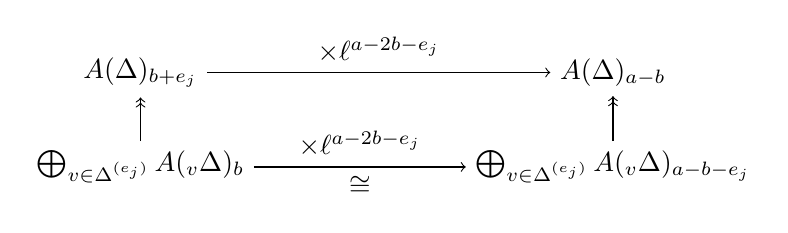
\begin{tikzpicture}[auto]
\node (a) at (0,1.2) {$A(\Delta)_{\bm{b}+\bm{e}_j}$}; 
\node (b) at (6,1.2) {$A(\Delta)_{\bm{a}-\bm{b}}$};
\node (c) at (0,0) {$\bigoplus_{v \in \Delta^{(\bm{e}_j)}} A(\lk_v \Delta)_{\bm{b}}$}; 
\node (d) at (6,0) {$\bigoplus_{v \in \Delta^{(\bm{e}_j)}} A(\lk_v \Delta)_{\bm{a}-\bm{b}-\bm{e}_j}$};
\draw[->] (a) to node {$\times \bm{\ell}^{\bm{a}-2\bm{b}-\bm{e}_j}$} (b);
\draw[->] (c) to node[above] {$\times \bm{\ell}^{\bm{a}-2\bm{b}-\bm{e}_j}$} node[below] {$\cong$} (d);
\draw[->>] (c) to (a);
\draw[->>] (d) to (b);
\end{tikzpicture}
\]
Here, the vertical maps are the composition of an isomorphism in Lemma~\ref{lem:cone} and a surjection in Lemma~\ref{lem:partition}.
For each $v \in \Delta^{(\bm{e}_j)}$, $(\lk_v \Delta,\kappa_{|V(\lk_\tau \Delta)})$ is an $(\bm{a}-\bm{e}_j)$-balanced homology sphere over $\mathbb{F}_2$. 
Thus, by Theorem~\ref{thm:main multiHL} and Remark~\ref{rem:Zariski}, the map
\[
\times \bm{\ell}^{\bm{a}-2\bm{b}-\bm{e}_j} :A(\lk_v \Delta)_{\bm{b}} \rightarrow A(\lk_v \Delta)_{\bm{a}-\bm{b}-\bm{e}_j}
\]
is an isomorphism for each $v \in \Delta^{(\bm{e}_j)}$.
The bottom horizontal map in the diagram is a direct sum of these isomorphisms, so it is an isomorphism. Thus the top horizontal map is surjective.
\end{proof}

We now derive a numerical consequence of Theorem~\ref{thm:manifold almost HL}, stated in Theorem~\ref{thm:manifold flag_h}.
Theorem~\ref{thm:manifold flag_h} is expressed in terms of flag $h''$-vectors, which is a suitable modification of flag $h$-vectors.
Given a field $\mathbbm{k}$, for an $\bm{a}$-balanced simplicial complex $(\Delta,\kappa)$, the \emph{flag $h'$-vector} $(h'_{\bm{b}})_{\bm{0} \leq \bm{b} \leq \bm{a}}$ and the \emph{flag $h''$-vector} $(h''_{\bm{b}})_{\bm{0} \leq \bm{b} \leq \bm{a}}$ of $(\Delta,\kappa)$ are defined as follows: 
\begin{align*}
h'_{\bm{b}}&=h_{\bm{b}} -\binom{\bm{a}}{\bm{b}} \left( \sum_{j=1}^{|\bm{b}|-1}(-1)^{|\bm{b}|-j}\widetilde{\beta}_{j-1} \right), \\
h''_{\bm{b}} &= 
    \begin{cases}
    h'_{\bm{b}} - \binom{\bm{a}}{\bm{b}} \widetilde{\beta}_{|\bm{b}|-1} & (\text{if } \bm{b} \neq \bm{a})\\
    h'_{\bm{b}} &(\text{if } \bm{b} = \bm{a})
    \end{cases}.
\end{align*}
Note that for a Cohen-Macaulay complex, both the flag $h'$-vector and flag $h''$-vector coincide with the flag $h$-vector.
For a $(d-1)$-dimensional simplicial complex, its \emph{$h'$-vector} $(h'_i)_{0 \leq i \leq d}$ (resp.~\emph{$h''$-vector} $(h''_i)_{0 \leq i \leq d}$) is defined as the flag $h'$-vector (resp.~flag $h''$-vector) considered as the monochromatic simplicial complex.
Note that the equalities $h'_i=\sum_{|\bm{b}|=i} h'_{\bm{b}}$ and $h''_i=\sum_{|\bm{b}|=i} h''_{\bm{b}}$ hold.

For homology manifolds, algebraic interpretations of $h'$- and $h''$-vectors are given by Schenzel~\cite{Sch81} and Novik and Swartz~\cite{NS09}.
The following lemma is the balanced analogue of these interpretations about flag $h'$- and $h''$-vectors.
A homology $(d-1)$-manifold $\Delta$ over $\mathbbm{k}$ is said to be \emph{orientable} if $\widetilde{\beta}_{d-1}$ equals the number of connected components of $\Delta$.
Recall that, for a graded $\mathbbm{k}[x_1,\ldots,x_n]$-module $M$, its socle is the submodule $\Soc(M)=\{a \in M: \mathfrak{m}a=0\}$, where $\mathfrak{m}=(x_1,\ldots,x_n)$ denotes the maximal graded ideal.
\begin{lemma} \label{lem:flag h', h''}
Let $(\Delta,\kappa)$ be an $\bm{a}$-balanced connected homology manifold over $\mathbbm{k}$ and let $\Theta$ be an $\mathbb{N}^m$-graded l.s.o.p.~for $\mathbbm{k}[\Delta]$.
Let $A=\mathbbm{k}[\Delta]/(\Theta)$ be an Artinian reduction of $\mathbbm{k}[\Delta]$ with respect to $\Theta$. Then,
\begin{enumerate}
\item[(i)] (Schenzel's formula~\cite[Theorem 3.1]{JMNS}) $h'_{\bm{b}}=\dim A_{\bm{b}}$ for each $\bm{b} \in \mathbb{N}^m$.
\item[(ii)] \cite[Corollary 3.3]{JMNS} $h''_{\bm{b}}=\dim A_{\bm{b}}/\Soc^\circ_{\bm{b}}$ for each $\bm{b} \in \mathbb{N}^m$, where $\Soc^\circ=\bigoplus_{\bm{0} \leq \bm{b} \lneq \bm{a}}\Soc(A)_{\bm{b}}$ denotes the internal socle of $A$.
\item[(iii)] (Dehn-Sommerville relation~\cite[Theorem 4.1]{JMNS}) If $\Delta$ is orientable, then $h''_{\bm{b}}=h''_{\bm{a}-\bm{b}}$ for each $\bm{b} \in \mathbb{N}^m$.
\end{enumerate}
\end{lemma}
We remark that every homology manifold over a field of characteristic $2$ is orientable.
Now we are ready to prove Theorem~\ref{thm:manifold flag_h}.
\begin{proof}[Proof of Theorem~\ref{thm:manifold flag_h}]
Let $\bm{b}, \bm{c} \in \mathbb{N}^m$ be integer vectors with $\bm{b} \lneq \bm{c} \lneq \bm{a}-\bm{b}$.
Then there exists some $j\in[m]$ such that $\bm{b}+\bm{e}_j \leq \bm{c}$.
By Theorem~\ref{thm:manifold almost HL}, the composition $A(\Delta)_{\bm{b}+\bm{e}_j} \overset{\times \bm{\ell}^{\bm{c}-\bm{b}-\bm{e}_j}}{\longrightarrow} A(\Delta)_{\bm{c}} \overset{\times \bm{\ell}^{\bm{a}-\bm{b}-\bm{c}}}{\longrightarrow} A(\Delta)_{\bm{a}-\bm{b}}$ is surjective, so the latter map $\times \bm{\ell}^{\bm{a}-\bm{b}-\bm{c}}:A(\Delta)_{\bm{c}} \rightarrow A(\Delta)_{\bm{a}-\bm{b}}$ is surjective.
Since $\bm{c} \lneq \bm{a}-\bm{b}$, the degree $\bm{c}$ component of the socle is contained in the kernel of this map. 
Thus by Lemma~\ref{lem:flag h', h''}, we have the inequality
\begin{equation}
h''_{\bm{c}}=\dim A(\Delta)_{\bm{c}} - \dim \Soc(A(\Delta))_{\bm{c}} \geq \dim A(\Delta)_{\bm{a}-\bm{b}} = h'_{\bm{a}-\bm{b}}. \label{eq:mfd_h}
\end{equation}
To complete the proof, we now convert (\ref{eq:mfd_h}) to an inequality between flag $h''$-vectors.
For this, if $\bm{b}\neq\bm{0}$, by Lemma~\ref{lem:flag h', h''} (iii), we have 
\begin{align}
h'_{\bm{a}-\bm{b}} &=h''_{\bm{a}-\bm{b}}+\binom{\bm{a}}{\bm{b}}\widetilde{\beta}_{|\bm{a}-\bm{b}|-1} & \notag \\
&=h''_{\bm{b}} + \binom{\bm{a}}{\bm{b}}\widetilde{\beta}_{|\bm{b}|} & (\widetilde{\beta}_{k}=\widetilde{\beta}_{d-k-1} \text{ for } k \geq 1 \text{ by Poincar\'{e} duality}), \label{eq:mfd_betti}
\end{align}
while the same equality (\ref{eq:mfd_betti}) also holds for $\bm{b}=\bm{0}$ since $h'_{\bm{a}}=1$ and $h''_{\bm{0}}+\binom{\bm{a}}{\bm{0}}\beta_{0}=1+0=1$. By (\ref{eq:mfd_h}) and (\ref{eq:mfd_betti}), the desired inequality $h''_{\bm{c}} \geq h''_{\bm{b}}+\binom{\bm{a}}{\bm{b}}\widetilde{\beta}_{|\bm{b}|}$ follows.
\end{proof}

\begin{coro} \label{cor:mfd-h}
For $\bm{a} \in \mathbb{N}^m_+$, let $(\Delta,\kappa)$ be an $\bm{a}$-balanced connected homology manifold over $\mathbb{F}_2$. Then, we have
\[
\frac{h_i''+\binom{d}{i}\widetilde{\beta}_{i}}{\binom{m+i-1}{i}} \leq \frac{h_{i+1}''}{\binom{m+i}{i+1}}
\]
for every nonnegative integer $i \in \mathbb{N}$ with $i\leq \min_{j=1}^m \frac{a_j-1}{2}$, where $d=|\bm{a}|$.
\end{coro}
\begin{proof}
The inequality between $h''$-vectors is derived by taking a weighted sum of the inequalities $h''_{\bm{b}} + \binom{\bm{a}}{\bm{b}}\widetilde{\beta}_{|\bm{b}|} \leq h''_{\bm{b}+\bm{e}_j}$ over all $\bm{b} \in \mathbb{N}^m$ with $|\bm{b}|=i$ and $j \in [m]$ as follows:
\begin{align*}
(m+i) \left(h''_i+\binom{d}{i}\widetilde{\beta}_i\right)
&=\sum_{|\bm{b}|=i}\sum_{j=1}^m (b_j+1)\left(h''_{\bm{b}}+\binom{\bm{a}}{\bm{b}}\widetilde{\beta}_i \right) \\
&\leq \sum_{|\bm{b}|=i}\sum_{j=1}^m (b_j+1)h''_{\bm{b}+\bm{e}_j}
=(i+1) h''_{i+1}. \qedhere
\end{align*}
\end{proof}

\subsection{Simplicial cycles}
For a $(d-1)$-dimensional simplicial complex $\Delta$ with $\widetilde{H}_{d-1}(\Delta;\mathbbm{k}) \neq 0$, we call a nonzero element $\mu \in \widetilde{H}_{d-1}(\Delta;\mathbbm{k})$ a \emph{simplicial cycle}.
Let $\Delta$ be a $(d-1)$-dimensional simplicial complex, and let $A=\mathbbm{k}[\Delta]/(\Theta)$ be an Artinian reduction of $\mathbbm{k}[\Delta]$.
A simplicial cycle $\mu$ of $\Delta$ induces a nonzero linear function $\Psi_\mu:A_{d} \rightarrow \mathbbm{k}$ by 
\begin{equation}
\Psi_\mu(x_\sigma) = \frac{\mu_\sigma}{[\sigma]} \label{eq:cycle}
\end{equation}
for each positively oriented facet $\sigma \in \Delta$, where $\mu_\sigma$ is the coefficient of a facet $\sigma$ and $[\sigma]$ is computed as in Lemma~\ref{lem:Lee formula}. Note that the linear function on $A_d$ is determined by the values of squarefree monomials~\cite[Theorem 9]{Lee}.
The existence of a linear map satisfying (\ref{eq:cycle}) for all facets of $\Delta$ can be verified by checking the equilibrium condition~\cite[Theorem 10]{Lee}. (Or alternatively consider weighted connected sum in the formulation of Karu-Xiao~\cite{KX}.)

A nonzero linear function $\varphi:\mathbbm{k}[\bm{x}]_d \rightarrow \mathbbm{k}$ determines a standard Artinian Gorenstein graded algebra $\mathbbm{k}[\bm{x}]/I$. Specifically, $f \in \mathbbm{k}[\bm{x}]_k$ is in $I$ if and only if $k \geq d+1$ or $\varphi(fg)=0$ for all $g \in \mathbbm{k}[\bm{x}]_{d-k}$.
Thus the map $\Psi_\mu$ (by concatenating a projection $\mathbbm{k}[\Delta]_{d} \twoheadrightarrow A_{d}$ to it) determines an Artinian Gorenstein $\mathbbm{k}$-algebra denoted as $B(\mu)$, which is called the \emph{Gorensteinification} of $A$~\cite{APP}.
Note that if $\Delta$ is a homology sphere, $A$ is itself Gorenstein, and hence we have $A=B(\mu)$ for any nonzero $\mu \in \widetilde{H}_{d-1}(\Delta;\mathbbm{k})$.
If $A$ is $\mathbb{N}^m$-graded, $B(\mu)$ is also $\mathbb{N}^m$-graded and satisfies the multigraded Poincar\'{e} duality.

Theorem~\ref{thm:main multiHL} is generalized to a simplicial cycle over a field of characteristic $2$ as follows.
\begin{theorem} \label{thm:simplicial cycle}
For an $\bm{a}$-balanced simplicial complex $(\Delta,\kappa)$, let $\mu$ be a simplicial cycle of $\Delta$ over a field $\mathbbm{k}$ of characteristic $2$.
Let $A=\widetilde{\mathbbm{k}}[\Delta]/(\Theta)$ be the generic $\mathbb{N}^m$-graded Artinian reduction of $\mathbbm{k}[\Delta]$ and let $B(\mu)$ be the Gorensteinification of $A$ with respect to $\mu$.
Then for generic elements $\ell_j \in B(\mu)_{\bm{e}_j}$, where $j=1,\ldots,m$, the multiplication map
\[
\times \bm{\ell}^{\bm{a}-2\bm{b}}: B(\mu)_{\bm{b}} \rightarrow B(\mu)_{\bm{a}-\bm{b}}
\]
is an isomorphism for every $\bm{b}\in\mathbb{N}^m$ with $\bm{b} \leq \frac{\bm{a}}{2}$.
\end{theorem}
\begin{proof}[Proof Sketch]
We provide only a proof sketch as the discussion is almost the same as in Sections 3-5.
Using a discussion similar to~\cite[Section 2.6]{KX}, by introducing the cone vertex, the simplicial cycle $\mu$ can be written as a weighted connected sum of simplex boundaries with the weights in $\mathbbm{k}$.
Accordingly, the map $\Psi_\mu$ is written as a weighted sum of the evaluation map of simplex boundaries. 
Hence, $\Psi=\Psi_\mu$ also satisfies the differential formula in Lemma~\ref{lem:diff}, and thus Corollary~\ref{cor:diff general}.
We can prove the desired statement for $B(\mu)$ in the same way as in the proof of Theorem~\ref{thm:main multiHL} since in the proof of Theorem~\ref{thm:main anis} we only used the fact that $A$ has the multigraded Poincar\'{e} duality, which is now passed to $B(\mu)$.
\end{proof}
\begin{rema}
To deduce a (generalized) lower bound type inequality from Theorem~\ref{thm:simplicial cycle}, it is imperative to understand the values $\dim A_*$ and $\dim B_*-\dim A_*$.
To the best of our knowledge, even in the natural $\mathbb{N}$-graded case, these numbers are not well understood outside of the setting of Buchsbaum complexes or homology manifolds. 
(See~\cite{Fog,Mu,NS12,NS20,Oba} for research in this direction.)
Further understanding of these numbers would also be valuable from the perspective of skeletal rigidity~\cite{TW}.
\end{rema}
From Theorem~\ref{thm:simplicial cycle}, we can obtain the following multigraded version of the top-heavy Lefschetz property for doubly Cohen-Macaulay complexes.
A simplicial complex $\Delta$ is called a \emph{doubly Cohen-Macaulay} complex (or a \emph{$2$-CM} complex) over a field $\mathbbm{k}$ if $\Delta$ is Cohen-Macaulay over $\mathbbm{k}$ and for each vertex $v$, $\Delta-v$ is Cohen-Macaulay over $\mathbbm{k}$ and has the same dimension as $\Delta$.
\begin{theorem} \label{thm:2CM lefschetz}
For $\bm{a} \in \mathbb{N}^m_+$, let $(\Delta,\kappa)$ be an $\bm{a}$-balanced doubly Cohen-Macaulay complex over a field $\mathbbm{k}$ of characteristic $2$.
Let $A=\widetilde{\mathbbm{k}}[\Delta]/(\Theta)$ be the generic $\mathbb{N}^m$-graded Artinian reduction of $\mathbbm{k}[\Delta]$.
Then, for generic elements $\ell_j \in A_{\bm{e}_j}$, where $j=1,\ldots,m$, the multiplication map
\[
\times \bm{\ell}^{\bm{a}-2\bm{b}}: A_{\bm{b}} \rightarrow A_{\bm{a}-\bm{b}}
\]
is injective for any $\bm{b} \in \mathbb{N}^m$ with $\bm{b} \leq \frac{\bm{a}}{2}$.
\end{theorem}
\begin{proof}
Let $d=|\bm{a}|$ and let $\mu_1,\ldots,\mu_k$ be a basis of $\widetilde{H}_{d-1}(\Delta;\mathbbm{k})$.
It is known that an Artinian reduction of the Stanley-Reisner ring of a doubly Cohen-Macaulay complex is a level ring~\cite[Section III.3]{Sta-book}, that is, $\Soc (A)=A_{\bm{a}}$.
This implies that for any nonzero $x \in A_{\bm{b}}$, there exists $y\in A_{\bm{a}-\bm{b}}$ such that $(\Psi_{\mu_1}(xy),\ldots,\Psi_{\mu_k}(xy))\neq0$.
Thus, the map $A(\Delta)_* \rightarrow \bigoplus_{i=1}^k B(\mu_i)_*$ is injective.
Consider the following commutative diagram:
\[
\begin{tikzpicture}[auto]
\node (a) at (0,1.2) {$A(\Delta)_{\bm{b}}$}; 
\node (b) at (4,1.2) {$A(\Delta)_{\bm{a}-\bm{b}}$};
\node (c) at (0,0) {$\bigoplus_{l=1}^k B(\mu_l)_{\bm{b}}$}; 
\node (d) at (4,0) {$\bigoplus_{l=1}^k B(\mu_l)_{\bm{a}-\bm{b}}$};
\draw[->] (a) to node {$\times \bm{\ell}^{\bm{a}-2\bm{b}}$} (b);
\draw[->] (c) to node[above] {$\times \bm{\ell}^{\bm{a}-2\bm{b}}$} node[below] {$\cong$} (d);
\draw[right hook->] (a) to (c);
\draw[right hook->] (b) to (d);
\end{tikzpicture}
\]
As the bottom map is an isomorphism by Theorem~\ref{thm:simplicial cycle}, the top map is injective.
\end{proof}
Now Theorem~\ref{thm:2CM_flag h} is readily derived.
\begin{proof}[Proof of Theorem~\ref{thm:2CM_flag h}]
For $\bm{b} \leq \bm{c} \leq \bm{a}-\bm{b}$, Theorem~\ref{thm:2CM lefschetz} implies that the linear map $\times \bm{\ell}^{\bm{b}-\bm{c}}:A_{\bm{b}} \rightarrow A_{\bm{c}}$ is injective. Thus $h_{\bm{b}}=\dim A_{\bm{b}} \leq \dim A_{\bm{c}} = h_{\bm{c}}$ follows.
\end{proof}
We remark that the inequality of $h$-vectors in Corollary~\ref{cor:h-vec} also follows by the same argument.

\section{Lefschetz property as an \texorpdfstring{$\mathbb{N}$}{N}-graded algebra}
Let $(\Delta,\kappa)$ be an $\bm{a}$-balanced simplicial complex for $\bm{a}\in\mathbb{N}_+^m$ with $d=|\bm{a}|$.
For simplicity, in this section, we focus on the case when $\Delta$ is a homology sphere.
Let $A$ be the generic $\mathbb{N}^m$-graded Artinian reduction of $\mathbbm{k}[\Delta]$.
Here, instead of considering $A$ as an $\mathbb{N}^m$-graded algebra, we regard $A$ as an $\mathbb{N}$-graded algebra $A=A_0\oplus\cdots\oplus A_d$ under the coarse grading $\deg x_v=1$ for all $v \in V(\Delta)$, and investigate the weak Lefschetz property as an $\mathbb{N}$-graded algebra.
See \cite[Conjecture 1.3]{CJMN} and \cite[Conjecture 1.1]{Oba} for related conjectures.

\subsection{Full-rankness at the ends}
From Theorem~\ref{thm:main multiHL}, one can deduce that, for a generic linear form $\ell \in A_1$, the multiplication map $\times \ell:A_i \rightarrow A_{i+1}$ is injective for $i \leq \min_{j=1}^m \frac{a_j-1}{2}$ and surjective for $i \geq d-1-\min_{j=1}^m \frac{a_j-1}{2}$.
We can slightly extend the range of $i$ as follows. 
\begin{theorem} \label{thm:fullrank at ends}
For $\bm{a} \in \mathbb{N}^m_+$ with $|\bm{a}|=d$, let $(\Delta,\kappa)$ be an $\bm{a}$-balanced homology $(d-1)$-sphere over $\mathbb{F}_2$ and let $\mathbbm{k}$ be a field of characteristic $0$ or $2$.
Let $A=\widetilde{\mathbbm{k}}[\Delta]/(\Theta)$ be the generic $\mathbb{N}^m$-graded Artinian reduction of $\mathbbm{k}[\Delta]$, and let $\ell=\sum_{v \in V(\Delta)} x_v \in A_1$.
Then the multiplication map $\times \ell:A_i \rightarrow A_{i+1}$ is injective for $i \leq \min \{ \frac{d-1}{2}, \frac{a_1}{2},\ldots,\frac{a_m}{2} \}$ and surjective for $i \geq d-1-\min\{ \frac{d-1}{2}, \frac{a_1}{2} ,\ldots, \frac{a_m}{2} \}$.
\end{theorem}
\begin{proof}
As the characteristic $0$ case follows from the characteristic $2$ case by an argument used in Section 6, we assume that $\mathbbm{k}$ is a field of characteristic $2$.
We first show the injectivity for $i \leq \min \{ \frac{d-1}{2}, \frac{a_1}{2},\ldots,\frac{a_m}{2} \}$.
For this, it suffices to show that the quadratic form $\mathcal{Q}:A_i \rightarrow A_{2i+1}$ defined by $\mathcal{Q}(g)=g^2 \ell$ satisfies the property that $\mathcal{Q}(g) \neq 0$ if $g \neq 0$.
Suppose that $g$ is a nonzero element in $A_i$.
Then by Poincar\'{e} duality (as an $\mathbb{N}$-graded algebra), there is a monomial $x_K$ of total degree $d-i$ such that $gx_K \neq 0$ in $A_d$.
Let $\bm{b}$ be the degree of the monomial $x_K$ in the $\mathbb{N}^m$-grading.
Then we have $\bm{0} \leq \bm{b} \leq \bm{a}$ and $|\bm{b}|=d-i$. 
Since $i \leq \min_{j \in [m]} \frac{a_j}{2}$, we have $\bm{b} \geq \frac{\bm{a}}{2}$. 
Because of this and $i \leq \frac{d-1}{2}$, the square $x_K^2$ can be written as $x_K^2=x_Ix_{v^*}x_J$ for some $\kappa$-transversal sequence $I$, some vertex $v^* \in V(\Delta)$, and some length $d-2i-1$ sequence $J$ of vertices.
We have the identity
\begin{align*}
\partial_I\Psi(\mathcal{Q}(g)x_J) &= \sum_{v \in V(\Delta)} \partial_I\Psi(g^2x_vx_J) \\
&=\sum_{v \in V(\Delta)} \Psi(g\sqrt{x_Ix_vx_J})^2 & (\text{by Corollary~\ref{cor:diff general}})\\
&\overset{(*)}{=}\Psi(g\sqrt{x_Ix_{v^*}x_J})^2 = \Psi(gx_K)^2 \neq 0,
\end{align*}
where $(*)$ follows from the uniqueness of a variable $x_u$ with $\sqrt{x_Ix_ux_J} \neq 0$ for fixed $I$ and $J$. Thus, we have $\mathcal{Q}(g) \neq 0$. Hence the desired injectivity is derived.

To prove the surjectivity, note that, by the Gorensteiness of $A$, $A_{d-i'}$ is a dual vector space of $A_{i'}$ for each $i'$.
Thus, the surjectivity of $\times \ell:A_{d-1-i} \rightarrow A_{d-i}$ is equivalent to the injectivity of $\times \ell :A_{i} \rightarrow A_{i+1}$.
Hence the desired surjectivity at the other end follows.
\end{proof}
\begin{rema}
    The assumption $i \leq \frac{d-1}{2}$ for the injectivity (and $i \geq \frac{d-1}{2}$ for the surjectivity) in Theorem~\ref{thm:fullrank at ends} is redundant when $m \geq 2$.
    For example, to compare Theorem~\ref{thm:fullrank at ends} with Theorem~\ref{thm:main multiHL}, if $(a_1,\ldots,a_m)=(2,\ldots,2)$ with $m \geq 2$, Theorem~\ref{thm:fullrank at ends} guarantees the injectivity of $\ell:A_1 \rightarrow A_2$, which does not follow directly from Theorem~\ref{thm:main multiHL}.
    See also~\cite{Oba} for a different proof for the injectivity of $\ell:A_1 \rightarrow A_2$.
\end{rema}
\subsection{Examples that fail the \texorpdfstring{$\mathbb{N}$}{N}-graded weak Lefschetz property}
In Theorem~\ref{thm:fullrank at ends}, we showed that $\times\ell:A_i \rightarrow A_{i+1}$ is generically full-rank at appropriate ends.
In contrast to~Theorem~\ref{thm:fullrank at ends}, we construct examples of an $\bm{a}$-balanced simplicial sphere such that the full-rankness generically fails around the middle degrees.
In~\cite{CJMN,Oba}, such an example was already obtained for $\bm{a}=(a_1,1)$ with $a_1 \geq 2$. Let us begin by recalling this construction.

The \emph{stellar subdivision} of $\Delta$ at a face $\sigma \in \Delta$ is the simplicial complex 
\begin{equation*}
(\Delta -\sigma) \cup \{\{v_\sigma\} \cup \tau: \tau \in \st_{\sigma}(\Delta), \tau \not\supset \sigma \},
\end{equation*} 
where $v_\sigma$ is a new vertex.
Note that stellar subdivisions preserve the underlying topological space.
Consider a stacked $a_1$-sphere, and apply stellar subdivisions to all of its facets. 
The resulting simplicial sphere $\Delta$ is stacked and $(a_1,1)$-balanced with the $2$-coloring $\kappa$ defined by $\kappa(v)=2$ if and only if $v$ is a new vertex.
It was shown in \cite{CJMN,Oba} that for any choice of an $\mathbb{N}^2$-graded l.s.o.p.~$\Theta$ of $\mathbbm{k}[\Delta]$, in the Artinian reduction $A=\mathbbm{k}[\Delta]/(\Theta)$, the map $\times\ell:A_1 \rightarrow A_2$ is degenerate for any $\ell \in A_1$.

To generalize this construction, we consider a partial barycentric subdivision~\cite{AW}.
We denote by $\Delta^{(i)}$ (resp.~$\Delta^{(\leq i)}$, $\Delta^{(\geq i)}$) the set of all faces of $\Delta$ of dimension equal to (resp.~at most, at least) $i$.
For a subset $\mathcal{S}$ of the power set of a finite set, the simplicial complex \emph{spanned by $\mathcal{S}$} is $\{T:T\subset S \text{ for some } S \in \mathcal{S}\}$.
For $0 \leq l < d$ and a pure $(d-1)$-dimensional simplicial complex $\Delta$, the \emph{$l$-th partial barycentric subdivision} $\sd^l(\Delta)$ of $\Delta$ is defined as follows: For each $\tau \in \Delta^{(\geq d-l)}$, let $v_{\tau}$ be a new vertex associated to $\tau$, and define $\sd^l(\Delta)$ as the simplicial complex spanned by the sets $\tau_0 \cup \{v_{\tau_1}, \ldots, v_{\tau_l}\}$ over all flags of faces $\tau_0 \subsetneq \tau_1 \subsetneq \cdots \subsetneq \tau_l$ of $\Delta$ with $\dim \tau_i=d-l-1+i$ for $i=0,\ldots,l$.
Note that we have $\sd^0(\Delta)=\Delta$ and $\sd^{d-1}(\Delta)$ coincides with the barycentric subdivision of $\Delta$. 
Equivalently, the $l$-th partial barycentric subdivision is obtained by ordering the faces of $\Delta^{(\geq d-l)}$ in decreasing order of dimension and then applying stellar subdivisions one by one.
As stellar subdivision preserves the underlying topological space, $\Delta$ and $\sd^l(\Delta)$ have the homeomorphic geometric realizations.
For a pure $(d-1)$-dimensional simplicial complex $\Delta$ and $l<d$, $\sd^l(\Delta)$ is $(d-l,\bm{1}_l)$-balanced with the coloring $\kappa:V(\sd^l(\Delta)) \rightarrow [l+1]$ defined by $\kappa(v)=1$ for $v \in V(\Delta)$ and $\kappa(v_\tau)=|\tau|-d+l+1$ for $v_\tau \in V(\sd^l(\Delta)) \setminus V(\Delta)$, where $\bm{1}_{l}$ is the all ones vector of length $l$.
By grouping the last $l$ colors of $\kappa$ into one color, one can consider $\sd^l(\Delta)$ as a $(d-l,l)$-balanced simplicial complex. We denote the resulting $2$-coloring by $\kappa^\circ$.

Our example is the $i$-th partial barycentric subdivision of a sphere with $h_i=h_{i+1}$. (Such a sphere is called $i$-stacked~\cite{MN}, and a stacked $(d-1)$-sphere is always $i$-stacked for $i < \lfloor d/2\rfloor $.)
More precisely, we have the following result. 
\begin{theorem} \label{thm:counterexample}
Let $\mathbbm{k}$ be an infinite field, and let $i, d$ be positive integers with $i < \frac{d}{2}$.
Let $\Delta$ be a simplicial $(d-1)$-sphere with $h_i(\Delta)=h_{i+1}(\Delta)$, and let $\sd^i(\Delta)$ be the $i$-th partial barycentric subdivision of $\Delta$ with the associated $2$-coloring $\kappa^\circ$.
Consider an l.s.o.p.~$\Theta=(\theta_1,\ldots,\theta_d)$ for $\mathbbm{k}[\sd^i(\Delta)]$ such that the $j$-th linear form $\theta_{j}$ is of degree $\bm{e}_2$ under the $\mathbb{N}^2$-grading induced by $\kappa^\circ$ for $j=d-i+1,\ldots,d$.
Then, for the Artinian reduction $A=\mathbbm{k}[\sd^i(\Delta)]/(\Theta)$ with respect to $\Theta$, the multiplication map $\times \ell:A_i \rightarrow A_{i+1}$ is degenerate for any linear form $\ell \in A_1$.

In particular, if $(\sd^i(\Delta),\kappa^\circ)$ is viewed as an $\bm{a}=(d-i,i)$-balanced simplicial complex, there is no $\mathbb{N}^2$-graded l.s.o.p.~$\Theta$ such that the Artinian reduction $\mathbbm{k}[\sd^i(\Delta)]/(\Theta)$ has the weak Lefschetz property as an $\mathbb{N}$-graded algebra.
\end{theorem}
\begin{proof}
As the geometric realizations of $\Delta$ and $\sd^i(\Delta)$ are homeomorphic, $\sd^i(\Delta)$ is a simplicial $(d-1)$-sphere.
As $\sd^i(\Delta)$ is obtained by a sequence of stellar subdivisions of faces of codimension at most $i$, we have $h_{i+1}(\sd^i(\Delta))-h_{i}(\sd^i(\Delta))=h_{i+1}(\Delta)-h_{i}(\Delta)=0$.
Hence $\dim A_i=h_{i}(\sd^i(\Delta))=h_{i+1}(\sd^i(\Delta))=\dim A_{i+1}$. 
Thus it suffices to prove that the multiplication map $\times \ell:A_i \rightarrow A_{i+1}$ cannot be surjective for any linear form $\ell \in A_1$.
Intuitively, from the perspective of skeletal rigidity~\cite{TW},
under the normalization $\ell=\sum_{v \in V(\sd^i(\Delta))} x_v$, the surjectivity of $\times \ell:A_i \rightarrow A_{i+1}$ is equivalent to the affine $i$-stress-freeness of the framework $(\sd^{i}(\Delta),p)$, where $p$ is the point configuration associated to $\Theta$. 
However the $(d-i)$-dimensional subframework induced by $V(\Delta)$ has the same $i$-skeleton as a $(d-1)$-sphere $\Delta$, so it must support an affine $i$-stress in $(d-i)$-dimension.
We now turn this geometric intuition into an algebraic proof.

Let $W=V(\Delta)$ be the vertex subset of $\sd^i(\Delta)$.
Consider the induced subcomplex $\sd^i(\Delta)_W=\{\tau \in \sd^i(\Delta):\tau \subset W\}$.
By definition, we have $\sd^i(\Delta)_W = \Delta^{(\leq d-i-1)}$.
Let $\pi:\mathbbm{k}[x_v : v \in V(\sd^i(\Delta))] \twoheadrightarrow \mathbbm{k}[x_v : v \in V(\Delta)]$ be the natural projection.
We have $\pi(\mathbbm{k}[\sd^i(\Delta)])=\mathbbm{k}[\sd^i(\Delta)_W]$ by definition and $\pi(\theta_{d-i+1})= \cdots= \pi(\theta_d)=0$ by the assumption. 
Thus for any $\ell \in A_1$ we have
\begin{align} 
&\dim \left(\mathbbm{k}[\sd^i(\Delta)]/(\Theta,\ell)\right)_{i+1} \label{eq:affine stress} \\
\geq& \left(\pi(\mathbbm{k}[\sd^i(\Delta)])/(\pi(\theta_1),\ldots,\pi(\theta_d),\pi(\ell)\right)_{i+1} \notag \\
 =& \left(\mathbbm{k}[\Delta^{(\leq d- i-1)}]/(\widetilde{\theta}_1,\ldots,\widetilde{\theta}_{d-i},\pi(\ell)\right)_{i+1} \notag \\
\overset{(*)}{\geq}& \dim \left(\mathbbm{k}[\Delta^{(\leq d-i-1)}]/(\widetilde{\theta}_1,\ldots,\widetilde{\theta}_{d-i})\right)_{i+1}- \dim \left(\mathbbm{k}[\Delta^{(\leq d- i-1)}]/(\widetilde{\theta}_1,\ldots,\widetilde{\theta}_{d-i})\right)_{i}, \label{eq:skeleton}
\end{align}
where we denote $\widetilde{\theta}_j=\pi(\theta_j)$, and the inequality ($*$) holds since $\pi(\ell)$ is a linear form.
Since the surjectivity of $\times\ell:A_i \rightarrow A_{i+1}$ is equivalent to the value (\ref{eq:affine stress}) being $0$, it suffices to prove that the value (\ref{eq:skeleton}) is positive.

To compute (\ref{eq:skeleton}), note that $(\widetilde{\theta}_1,\ldots,\widetilde{\theta}_{d-i})$ is an l.s.o.p.~for $\mathbbm{k}[\Delta^{(\leq d-i-1)}]$. 
This follows from the Kind-Kleinschmidt's criterion~\cite[Lemma III.2.4]{Sta-book}.
Observe also that $\Delta^{(\leq d - i-1)}$ is Cohen-Macaulay as $\Delta$ is Cohen-Macaulay\footnote{For example, homological condition of Cohen-Macaulayness can be directly checked as follows. For each $\tau \in \Delta^{(\leq d- i-1)}$, $\lk_\tau(\Delta^{(\leq d- i-1)}) =(\lk_\tau \Delta )^{\leq (d-i-|\tau| -1)}$ holds. So $\widetilde{H}_j(\lk_\tau(\Delta^{(\leq d- i-1)});\mathbbm{k})=\widetilde{H}_j(\lk_\tau \Delta;\mathbbm{k})=0$ for $j \leq d-i-|\tau|-2$.}.
Thus we have
\[
\dim \left(\mathbbm{k}[\Delta^{(\leq d- i-1)}]/(\widetilde{\theta}_1,\ldots,\widetilde{\theta}_{d-i}\right)_{j}=
h_{j}(\Delta^{(\leq d-i-1)}) \qquad \text{ for } j=0,\ldots,d-i.
\]
Now in the Stanley's triangle table for $\Delta$ (see~\cite[p.250]{Zie}), the $h$-vector of $\Delta^{(\leq d-i-1)}$ appears in the $(d-i)$-th row. So the consecutive difference $h_{i+1}(\Delta^{(\leq d-i-1)})-h_{i}(\Delta^{(\leq d-i-1)})$ appears in the $(d-i+1)$-th row. As the $h$-vector of $\sd^i(\Delta)$ is positive, all the entries in the triangle table are positive. Thus, (\ref{eq:skeleton}) is positive. 
We thus verified the degeneracy of $\times\ell:A_i \rightarrow A_{i+1}$.
\end{proof}


 
